% Options for packages loaded elsewhere
\PassOptionsToPackage{unicode}{hyperref}
\PassOptionsToPackage{hyphens}{url}
%
\documentclass[
]{article}
\usepackage{amsmath,amssymb}
\usepackage{lmodern}
\usepackage{iftex}
\ifPDFTeX
  \usepackage[T1]{fontenc}
  \usepackage[utf8]{inputenc}
  \usepackage{textcomp} % provide euro and other symbols
\else % if luatex or xetex
  \usepackage{unicode-math}
  \defaultfontfeatures{Scale=MatchLowercase}
  \defaultfontfeatures[\rmfamily]{Ligatures=TeX,Scale=1}
\fi
% Use upquote if available, for straight quotes in verbatim environments
\IfFileExists{upquote.sty}{\usepackage{upquote}}{}
\IfFileExists{microtype.sty}{% use microtype if available
  \usepackage[]{microtype}
  \UseMicrotypeSet[protrusion]{basicmath} % disable protrusion for tt fonts
}{}
\makeatletter
\@ifundefined{KOMAClassName}{% if non-KOMA class
  \IfFileExists{parskip.sty}{%
    \usepackage{parskip}
  }{% else
    \setlength{\parindent}{0pt}
    \setlength{\parskip}{6pt plus 2pt minus 1pt}}
}{% if KOMA class
  \KOMAoptions{parskip=half}}
\makeatother
\usepackage{xcolor}
\usepackage[margin=1in]{geometry}
\usepackage{color}
\usepackage{fancyvrb}
\newcommand{\VerbBar}{|}
\newcommand{\VERB}{\Verb[commandchars=\\\{\}]}
\DefineVerbatimEnvironment{Highlighting}{Verbatim}{commandchars=\\\{\}}
% Add ',fontsize=\small' for more characters per line
\usepackage{framed}
\definecolor{shadecolor}{RGB}{248,248,248}
\newenvironment{Shaded}{\begin{snugshade}}{\end{snugshade}}
\newcommand{\AlertTok}[1]{\textcolor[rgb]{0.94,0.16,0.16}{#1}}
\newcommand{\AnnotationTok}[1]{\textcolor[rgb]{0.56,0.35,0.01}{\textbf{\textit{#1}}}}
\newcommand{\AttributeTok}[1]{\textcolor[rgb]{0.77,0.63,0.00}{#1}}
\newcommand{\BaseNTok}[1]{\textcolor[rgb]{0.00,0.00,0.81}{#1}}
\newcommand{\BuiltInTok}[1]{#1}
\newcommand{\CharTok}[1]{\textcolor[rgb]{0.31,0.60,0.02}{#1}}
\newcommand{\CommentTok}[1]{\textcolor[rgb]{0.56,0.35,0.01}{\textit{#1}}}
\newcommand{\CommentVarTok}[1]{\textcolor[rgb]{0.56,0.35,0.01}{\textbf{\textit{#1}}}}
\newcommand{\ConstantTok}[1]{\textcolor[rgb]{0.00,0.00,0.00}{#1}}
\newcommand{\ControlFlowTok}[1]{\textcolor[rgb]{0.13,0.29,0.53}{\textbf{#1}}}
\newcommand{\DataTypeTok}[1]{\textcolor[rgb]{0.13,0.29,0.53}{#1}}
\newcommand{\DecValTok}[1]{\textcolor[rgb]{0.00,0.00,0.81}{#1}}
\newcommand{\DocumentationTok}[1]{\textcolor[rgb]{0.56,0.35,0.01}{\textbf{\textit{#1}}}}
\newcommand{\ErrorTok}[1]{\textcolor[rgb]{0.64,0.00,0.00}{\textbf{#1}}}
\newcommand{\ExtensionTok}[1]{#1}
\newcommand{\FloatTok}[1]{\textcolor[rgb]{0.00,0.00,0.81}{#1}}
\newcommand{\FunctionTok}[1]{\textcolor[rgb]{0.00,0.00,0.00}{#1}}
\newcommand{\ImportTok}[1]{#1}
\newcommand{\InformationTok}[1]{\textcolor[rgb]{0.56,0.35,0.01}{\textbf{\textit{#1}}}}
\newcommand{\KeywordTok}[1]{\textcolor[rgb]{0.13,0.29,0.53}{\textbf{#1}}}
\newcommand{\NormalTok}[1]{#1}
\newcommand{\OperatorTok}[1]{\textcolor[rgb]{0.81,0.36,0.00}{\textbf{#1}}}
\newcommand{\OtherTok}[1]{\textcolor[rgb]{0.56,0.35,0.01}{#1}}
\newcommand{\PreprocessorTok}[1]{\textcolor[rgb]{0.56,0.35,0.01}{\textit{#1}}}
\newcommand{\RegionMarkerTok}[1]{#1}
\newcommand{\SpecialCharTok}[1]{\textcolor[rgb]{0.00,0.00,0.00}{#1}}
\newcommand{\SpecialStringTok}[1]{\textcolor[rgb]{0.31,0.60,0.02}{#1}}
\newcommand{\StringTok}[1]{\textcolor[rgb]{0.31,0.60,0.02}{#1}}
\newcommand{\VariableTok}[1]{\textcolor[rgb]{0.00,0.00,0.00}{#1}}
\newcommand{\VerbatimStringTok}[1]{\textcolor[rgb]{0.31,0.60,0.02}{#1}}
\newcommand{\WarningTok}[1]{\textcolor[rgb]{0.56,0.35,0.01}{\textbf{\textit{#1}}}}
\usepackage{longtable,booktabs,array}
\usepackage{calc} % for calculating minipage widths
% Correct order of tables after \paragraph or \subparagraph
\usepackage{etoolbox}
\makeatletter
\patchcmd\longtable{\par}{\if@noskipsec\mbox{}\fi\par}{}{}
\makeatother
% Allow footnotes in longtable head/foot
\IfFileExists{footnotehyper.sty}{\usepackage{footnotehyper}}{\usepackage{footnote}}
\makesavenoteenv{longtable}
\usepackage{graphicx}
\makeatletter
\def\maxwidth{\ifdim\Gin@nat@width>\linewidth\linewidth\else\Gin@nat@width\fi}
\def\maxheight{\ifdim\Gin@nat@height>\textheight\textheight\else\Gin@nat@height\fi}
\makeatother
% Scale images if necessary, so that they will not overflow the page
% margins by default, and it is still possible to overwrite the defaults
% using explicit options in \includegraphics[width, height, ...]{}
\setkeys{Gin}{width=\maxwidth,height=\maxheight,keepaspectratio}
% Set default figure placement to htbp
\makeatletter
\def\fps@figure{htbp}
\makeatother
\setlength{\emergencystretch}{3em} % prevent overfull lines
\providecommand{\tightlist}{%
  \setlength{\itemsep}{0pt}\setlength{\parskip}{0pt}}
\setcounter{secnumdepth}{-\maxdimen} % remove section numbering
\usepackage{booktabs}
\usepackage{longtable}
\usepackage{array}
\usepackage{multirow}
\usepackage{wrapfig}
\usepackage{float}
\usepackage{colortbl}
\usepackage{pdflscape}
\usepackage{tabu}
\usepackage{threeparttable}
\usepackage{threeparttablex}
\usepackage[normalem]{ulem}
\usepackage{makecell}
\usepackage{xcolor}
\ifLuaTeX
  \usepackage{selnolig}  % disable illegal ligatures
\fi
\IfFileExists{bookmark.sty}{\usepackage{bookmark}}{\usepackage{hyperref}}
\IfFileExists{xurl.sty}{\usepackage{xurl}}{} % add URL line breaks if available
\urlstyle{same} % disable monospaced font for URLs
\hypersetup{
  pdftitle={Trabajo},
  pdfauthor={Héctor García Hernández y David Andreu Roqueta},
  hidelinks,
  pdfcreator={LaTeX via pandoc}}

\title{Trabajo}
\author{Héctor García Hernández y David Andreu Roqueta}
\date{2023-10-08}

\begin{document}
\maketitle

\hypertarget{librerias-utilizadas}{%
\subsection{Librerias utilizadas}\label{librerias-utilizadas}}

\begin{verbatim}
## Warning: package 'readxl' was built under R version 4.2.3
\end{verbatim}

\begin{verbatim}
## Warning: package 'plm' was built under R version 4.2.3
\end{verbatim}

\begin{verbatim}
## Warning: package 'forecast' was built under R version 4.2.3
\end{verbatim}

\begin{verbatim}
## Registered S3 method overwritten by 'quantmod':
##   method            from
##   as.zoo.data.frame zoo
\end{verbatim}

\begin{verbatim}
## 
## Attaching package: 'dplyr'
\end{verbatim}

\begin{verbatim}
## The following objects are masked from 'package:plm':
## 
##     between, lag, lead
\end{verbatim}

\begin{verbatim}
## The following objects are masked from 'package:stats':
## 
##     filter, lag
\end{verbatim}

\begin{verbatim}
## The following objects are masked from 'package:base':
## 
##     intersect, setdiff, setequal, union
\end{verbatim}

\begin{verbatim}
## Warning: package 'ggplot2' was built under R version 4.2.3
\end{verbatim}

\begin{Shaded}
\begin{Highlighting}[]
\CommentTok{\# Función para convertir el trimestre a fecha}
\NormalTok{convertir\_a\_fecha }\OtherTok{\textless{}{-}} \ControlFlowTok{function}\NormalTok{(trimestre) \{}
\NormalTok{  año }\OtherTok{\textless{}{-}} \FunctionTok{substr}\NormalTok{(trimestre, }\DecValTok{1}\NormalTok{, }\DecValTok{4}\NormalTok{)}
\NormalTok{  t }\OtherTok{\textless{}{-}} \FunctionTok{substr}\NormalTok{(trimestre, }\DecValTok{6}\NormalTok{, }\DecValTok{6}\NormalTok{)}
  
  \CommentTok{\# Definir el mes de inicio para cada trimestre}
\NormalTok{  mes\_inicio }\OtherTok{\textless{}{-}} \FunctionTok{ifelse}\NormalTok{(t }\SpecialCharTok{==} \StringTok{"1"}\NormalTok{, }\StringTok{"01"}\NormalTok{, }
                       \FunctionTok{ifelse}\NormalTok{(t }\SpecialCharTok{==} \StringTok{"2"}\NormalTok{, }\StringTok{"04"}\NormalTok{, }
                              \FunctionTok{ifelse}\NormalTok{(t }\SpecialCharTok{==} \StringTok{"3"}\NormalTok{, }\StringTok{"07"}\NormalTok{, }\StringTok{"10"}\NormalTok{)))}
  
\NormalTok{  fecha }\OtherTok{=} \FunctionTok{as.Date}\NormalTok{(}\FunctionTok{paste}\NormalTok{(año, mes\_inicio, }\StringTok{"01"}\NormalTok{, }\AttributeTok{sep =} \StringTok{"{-}"}\NormalTok{))}
  \FunctionTok{return}\NormalTok{(}\FunctionTok{format}\NormalTok{(fecha, }\StringTok{"\%Y{-}\%m{-}\%d"}\NormalTok{))}
\NormalTok{\}}
\end{Highlighting}
\end{Shaded}

\hypertarget{introducciuxf3n}{%
\section{Introducción}\label{introducciuxf3n}}

Hoy en día la accesibilidad a la vivienda es un problema presente en
nuestra sociedad. Nosotros vamos a intentar analizarlo desde el punto de
vista del precio de la vivienda.

\hypertarget{preguntas}{%
\subsection{Preguntas}\label{preguntas}}

¿Como se comporta el precio de la vivienda? ¿Como se relaciona el precio
de la vivienda con el IPC, las personas activas y el coste salarial?
¿Cual va a ser el precio de la vivienda el trimestre que viene y el
siguiente?

\hypertarget{anuxe1lisis-de-datos-de-panel}{%
\section{Análisis de datos de
panel}\label{anuxe1lisis-de-datos-de-panel}}

\hypertarget{descripciuxf3n-de-los-datos}{%
\subsection{Descripción de los
datos}\label{descripciuxf3n-de-los-datos}}

En nuestro archivo datos\_trabajo.xlsx, tenemos un total de 204
observaciones y 6 variables. Las variables se definen de la siguiente
forma:

\begin{itemize}
\tightlist
\item
  CCAA: comunidad autónoma (individuos) (no tenemos datos ni de Ceuta ni
  de Melilla)
\item
  Periodo: periodo de tiempo, desde 2017 hasta 2020 divididos por
  trimestres
\item
  IPC: índices de precio de consumo
\item
  Personas activas: el número de personas activas
\item
  Precio vivienda: es un índice confeccionado en España por el Instituto
  Nacional de Estadística que fue publicado con el propósito de reflejar
  la evolución de precios de la vivienda.
\item
  Coste\_salarial\_total: se refiere al gasto total que una empresa
  incurre al pagar los salarios y las prestaciones a sus empleados. Se
  incluyen los sectores de industria, construcción y servicios
\end{itemize}

Destacar que son datos de panel ya que contienen una serie temporal por
cada unidad de unos datos de corte transversal. Al ser datos de panel
tenemos individuos (CCAA) y el periodo de tiempo (periodo) y el número
de observaciones coincide con el resultado de multiplicar el número de
periodos de tiempo por el número de individuos 17x12=204 que son
nuestras observaciones.

La pregunta a la que responderemos con estos datos es si influyen y en
el caso de que influyan de que forma, el ipc, el coste salarial total y
el número de personas activas sobre el precio de la vivienda.

\hypertarget{carga-de-datos}{%
\subsection{Carga de datos}\label{carga-de-datos}}

Abrimos nuestro fichero de datos y cargamos los datos en un panel data
frame. Le especificamos los dos índices que son la comundiad autónoma
(CCAA) y el periodo de tiempo (Periodo)

\begin{Shaded}
\begin{Highlighting}[]
\NormalTok{datos }\OtherTok{\textless{}{-}} \FunctionTok{read\_excel}\NormalTok{(}\StringTok{"./datos\_trabajo.xlsx"}\NormalTok{)}
\NormalTok{data }\OtherTok{\textless{}{-}} \FunctionTok{pdata.frame}\NormalTok{(datos, }\AttributeTok{index =} \FunctionTok{c}\NormalTok{(}\StringTok{"CCAA"}\NormalTok{,}\StringTok{"Periodo"}\NormalTok{), }\AttributeTok{drop.index =} \ConstantTok{FALSE}\NormalTok{, }\AttributeTok{row.names =} \ConstantTok{TRUE}\NormalTok{)}

\CommentTok{\# Convertimos a numérico las columnas Personas\_activas y Precio\_vivienda que estaban en tipo texto y cambiamos el nombre de la columna Coste.salarial.total a Coste\_salarial\_total.}
\NormalTok{data}\SpecialCharTok{$}\NormalTok{Personas\_activas }\OtherTok{=} \FunctionTok{as.numeric}\NormalTok{(data}\SpecialCharTok{$}\NormalTok{Personas\_activas)}
\NormalTok{data}\SpecialCharTok{$}\NormalTok{Precio\_vivienda }\OtherTok{=} \FunctionTok{as.numeric}\NormalTok{(data}\SpecialCharTok{$}\NormalTok{Precio\_vivienda)}
\FunctionTok{colnames}\NormalTok{(data)[}\FunctionTok{colnames}\NormalTok{(data) }\SpecialCharTok{==} \StringTok{"Coste.salarial.total"}\NormalTok{] }\OtherTok{\textless{}{-}} \StringTok{"Coste\_salarial\_total"}

\FunctionTok{head}\NormalTok{(data)}
\end{Highlighting}
\end{Shaded}

\begin{verbatim}
##                       CCAA Periodo      IPC Personas_activas Precio_vivienda
## Andalucía-2017T1 Andalucía  2017T1 94.47567           3980.8         104.051
## Andalucía-2017T2 Andalucía  2017T2 95.31533           3962.1         105.676
## Andalucía-2017T3 Andalucía  2017T3 94.67267           3957.9         106.913
## Andalucía-2017T4 Andalucía  2017T4 96.26667           3932.2         107.763
## Andalucía-2018T1 Andalucía  2018T1 95.32267           3943.4         108.283
## Andalucía-2018T2 Andalucía  2018T2 97.00000           3942.7         110.695
##                  Coste.laboral.total Coste_salarial_total
## Andalucía-2017T1             2199.80              1602.09
## Andalucía-2017T2             2340.30              1743.40
## Andalucía-2017T3             2225.59              1632.62
## Andalucía-2017T4             2362.04              1768.78
## Andalucía-2018T1             2159.14              1573.94
## Andalucía-2018T2             2297.25              1712.06
\end{verbatim}

Convertimos a numérico las columnas Personas\_activas y Precio\_vivienda
que estaban en tipo texto y cambiamos el nombre de la columna
Coste.salarial.total a Coste\_salarial\_total.

\hypertarget{anuxe1lisis-exploratorio}{%
\subsection{Análisis exploratorio}\label{anuxe1lisis-exploratorio}}

Lo primero que vamos a hacer es ver el comportamiento de los datos que
manejamos. A continuación, observamos la evolución de la media para
todas las comunidades de nuestras variables a lo largo del tiempo.

\begin{Shaded}
\begin{Highlighting}[]
\CommentTok{\# Calcular la media de cada variable por periodo}
\NormalTok{medias\_por\_periodo }\OtherTok{\textless{}{-}}\NormalTok{ data }\SpecialCharTok{\%\textgreater{}\%}
  \FunctionTok{group\_by}\NormalTok{(Periodo) }\SpecialCharTok{\%\textgreater{}\%}
  \FunctionTok{summarise}\NormalTok{(}
    \AttributeTok{Media\_IPC =} \FunctionTok{mean}\NormalTok{(IPC, }\AttributeTok{na.rm =} \ConstantTok{TRUE}\NormalTok{),}
    \AttributeTok{Media\_Personas\_Activas =} \FunctionTok{mean}\NormalTok{(Personas\_activas, }\AttributeTok{na.rm =} \ConstantTok{TRUE}\NormalTok{),}
    \AttributeTok{Media\_Precio\_Vivienda =} \FunctionTok{mean}\NormalTok{(Precio\_vivienda, }\AttributeTok{na.rm =} \ConstantTok{TRUE}\NormalTok{),}
    \AttributeTok{Media\_Coste\_Salarial\_Total =} \FunctionTok{mean}\NormalTok{(Coste\_salarial\_total, }\AttributeTok{na.rm =} \ConstantTok{TRUE}\NormalTok{)}
\NormalTok{  )}

\NormalTok{medias\_por\_periodo}\SpecialCharTok{$}\NormalTok{Periodo }\OtherTok{\textless{}{-}} \FunctionTok{sapply}\NormalTok{(}\FunctionTok{as.character}\NormalTok{(medias\_por\_periodo}\SpecialCharTok{$}\NormalTok{Periodo), convertir\_a\_fecha)}
\NormalTok{medias\_por\_periodo}\SpecialCharTok{$}\NormalTok{Periodo }\OtherTok{=} \FunctionTok{as.Date}\NormalTok{(medias\_por\_periodo}\SpecialCharTok{$}\NormalTok{Periodo)}

\CommentTok{\# Crear los gráficos}
\NormalTok{p1 }\OtherTok{\textless{}{-}} \FunctionTok{ggplot}\NormalTok{(medias\_por\_periodo, }\FunctionTok{aes}\NormalTok{(}\AttributeTok{x =}\NormalTok{ Periodo, }\AttributeTok{y =}\NormalTok{ Media\_IPC)) }\SpecialCharTok{+}
  \FunctionTok{geom\_line}\NormalTok{() }\SpecialCharTok{+}
  \FunctionTok{theme\_minimal}\NormalTok{() }\SpecialCharTok{+}
  \FunctionTok{ggtitle}\NormalTok{(}\StringTok{"Evolución Media del IPC"}\NormalTok{)}

\NormalTok{p2 }\OtherTok{\textless{}{-}} \FunctionTok{ggplot}\NormalTok{(medias\_por\_periodo, }\FunctionTok{aes}\NormalTok{(}\AttributeTok{x =}\NormalTok{ Periodo, }\AttributeTok{y =}\NormalTok{ Media\_Personas\_Activas)) }\SpecialCharTok{+}
  \FunctionTok{geom\_line}\NormalTok{() }\SpecialCharTok{+}
  \FunctionTok{theme\_minimal}\NormalTok{() }\SpecialCharTok{+}
  \FunctionTok{ggtitle}\NormalTok{(}\StringTok{"Evolución de Personas Activas"}\NormalTok{)}

\NormalTok{p3 }\OtherTok{\textless{}{-}} \FunctionTok{ggplot}\NormalTok{(medias\_por\_periodo, }\FunctionTok{aes}\NormalTok{(}\AttributeTok{x =}\NormalTok{ Periodo, }\AttributeTok{y =}\NormalTok{ Media\_Precio\_Vivienda)) }\SpecialCharTok{+}
  \FunctionTok{geom\_line}\NormalTok{() }\SpecialCharTok{+}
  \FunctionTok{theme\_minimal}\NormalTok{() }\SpecialCharTok{+}
  \FunctionTok{ggtitle}\NormalTok{(}\StringTok{"Evolución del Precio de Vivienda"}\NormalTok{)}

\NormalTok{p4 }\OtherTok{\textless{}{-}} \FunctionTok{ggplot}\NormalTok{(medias\_por\_periodo, }\FunctionTok{aes}\NormalTok{(}\AttributeTok{x =}\NormalTok{ Periodo, }\AttributeTok{y =}\NormalTok{ Media\_Coste\_Salarial\_Total)) }\SpecialCharTok{+}
  \FunctionTok{geom\_line}\NormalTok{() }\SpecialCharTok{+}
  \FunctionTok{theme\_minimal}\NormalTok{() }\SpecialCharTok{+}
  \FunctionTok{ggtitle}\NormalTok{(}\StringTok{"Evolución del Coste Salarial Total"}\NormalTok{)}

\CommentTok{\# Mostrar los gráficos en un grid}
\FunctionTok{library}\NormalTok{(gridExtra)}
\end{Highlighting}
\end{Shaded}

\begin{verbatim}
## Warning: package 'gridExtra' was built under R version 4.2.3
\end{verbatim}

\begin{verbatim}
## 
## Attaching package: 'gridExtra'
\end{verbatim}

\begin{verbatim}
## The following object is masked from 'package:dplyr':
## 
##     combine
\end{verbatim}

\begin{Shaded}
\begin{Highlighting}[]
\FunctionTok{grid.arrange}\NormalTok{(p1, p2, p3, p4, }\AttributeTok{ncol =} \DecValTok{2}\NormalTok{)}
\end{Highlighting}
\end{Shaded}

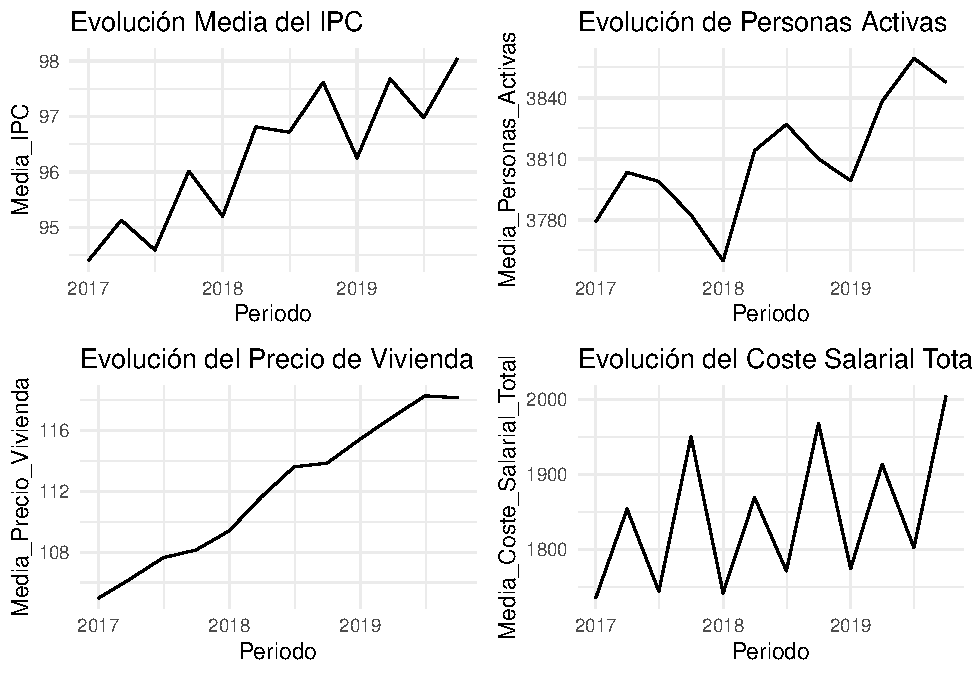
\includegraphics{trabajo_files/figure-latex/unnamed-chunk-4-1.pdf}

\begin{enumerate}
\def\labelenumi{\arabic{enumi}.}
\item
  \textbf{Evolución Media del IPC}: El IPC muestra fluctuaciones a lo
  largo del tiempo, con un leve aumento en la tendencia. Como medida de
  la inflación, un aumento en el IPC podría influir en el poder
  adquisitivo y, por tanto, en la capacidad de los consumidores para
  comprar viviendas.
\item
  \textbf{Evolución de Personas Activas}: Hay una tendencia general
  ascendente en el número de personas activas, lo que puede estar
  relacionado con una economía en crecimiento. Un aumento en la fuerza
  laboral activa podría correlacionarse con una mayor demanda de
  vivienda, ya que más personas podrían tener los medios para comprar o
  alquilar.
\item
  \textbf{Evolución del Precio de Vivienda}: Esta línea muestra una
  tendencia claramente ascendente, lo que indica un incremento constante
  en el precio de la vivienda. Esta variable es el foco principal del
  análisis y es la única que no presenta un patrón estacional.
\item
  \textbf{Evolución del Coste Salarial Total}: El coste salarial total
  también presenta una tendencia al alza, lo cual podría interpretarse
  como un aumento en los costos para las empresas. Aunque esta variable
  no se relaciona directamente con el mercado de la vivienda, los
  salarios más altos podrían aumentar la capacidad de los trabajadores
  para adquirir viviendas, afectando así la demanda y, posiblemente, los
  precios.
\end{enumerate}

Cabe destacar que el patrón estacional del coste salarial y de la
evolución del PIB es similar, ambos presentan una forma de M cada año,
en cambio la evolución de personas activas es más parecido a una U
invertida, con su pico en el segundo o tercer trimestre del año.

\begin{Shaded}
\begin{Highlighting}[]
\CommentTok{\# Calcular la media de cada variable por CCAA}
\NormalTok{medias\_por\_CCAA }\OtherTok{\textless{}{-}}\NormalTok{ data }\SpecialCharTok{\%\textgreater{}\%}
  \FunctionTok{group\_by}\NormalTok{(CCAA) }\SpecialCharTok{\%\textgreater{}\%}
  \FunctionTok{summarise}\NormalTok{(}
    \AttributeTok{Media\_IPC =} \FunctionTok{mean}\NormalTok{(IPC, }\AttributeTok{na.rm =} \ConstantTok{TRUE}\NormalTok{),}
    \AttributeTok{Media\_Personas\_Activas =} \FunctionTok{mean}\NormalTok{(Personas\_activas, }\AttributeTok{na.rm =} \ConstantTok{TRUE}\NormalTok{),}
    \AttributeTok{Media\_Precio\_Vivienda =} \FunctionTok{mean}\NormalTok{(Precio\_vivienda, }\AttributeTok{na.rm =} \ConstantTok{TRUE}\NormalTok{),}
    \AttributeTok{Media\_Coste\_Salarial\_Total =} \FunctionTok{mean}\NormalTok{(Coste\_salarial\_total, }\AttributeTok{na.rm =} \ConstantTok{TRUE}\NormalTok{)}
\NormalTok{  )}

\NormalTok{p1 }\OtherTok{\textless{}{-}} \FunctionTok{ggplot}\NormalTok{(medias\_por\_CCAA, }\FunctionTok{aes}\NormalTok{(}\AttributeTok{x =}\NormalTok{ CCAA, }\AttributeTok{y =}\NormalTok{ Media\_IPC)) }\SpecialCharTok{+}
  \FunctionTok{geom\_bar}\NormalTok{(}\AttributeTok{stat =} \StringTok{\textquotesingle{}identity\textquotesingle{}}\NormalTok{) }\SpecialCharTok{+}
  \FunctionTok{theme\_minimal}\NormalTok{() }\SpecialCharTok{+}
  \FunctionTok{ggtitle}\NormalTok{(}\StringTok{"Media del IPC por CCAA"}\NormalTok{) }\SpecialCharTok{+}
  \FunctionTok{theme}\NormalTok{(}\AttributeTok{axis.text.x =} \FunctionTok{element\_blank}\NormalTok{(), }
        \AttributeTok{axis.ticks.x =} \FunctionTok{element\_blank}\NormalTok{())}


\NormalTok{p2 }\OtherTok{\textless{}{-}} \FunctionTok{ggplot}\NormalTok{(medias\_por\_CCAA, }\FunctionTok{aes}\NormalTok{(}\AttributeTok{x =}\NormalTok{ CCAA, }\AttributeTok{y =}\NormalTok{ Media\_Personas\_Activas)) }\SpecialCharTok{+}
  \FunctionTok{geom\_bar}\NormalTok{(}\AttributeTok{stat =} \StringTok{\textquotesingle{}identity\textquotesingle{}}\NormalTok{) }\SpecialCharTok{+}
  \FunctionTok{theme\_minimal}\NormalTok{() }\SpecialCharTok{+}
  \FunctionTok{ggtitle}\NormalTok{(}\StringTok{"Personas Activas por CCAA"}\NormalTok{) }\SpecialCharTok{+}
  \FunctionTok{theme}\NormalTok{(}\AttributeTok{axis.text.x =} \FunctionTok{element\_blank}\NormalTok{(), }
        \AttributeTok{axis.ticks.x =} \FunctionTok{element\_blank}\NormalTok{())}

\NormalTok{p3 }\OtherTok{\textless{}{-}} \FunctionTok{ggplot}\NormalTok{(medias\_por\_CCAA, }\FunctionTok{aes}\NormalTok{(}\AttributeTok{x =}\NormalTok{ CCAA, }\AttributeTok{y =}\NormalTok{ Media\_Precio\_Vivienda)) }\SpecialCharTok{+}
  \FunctionTok{geom\_bar}\NormalTok{(}\AttributeTok{stat =} \StringTok{\textquotesingle{}identity\textquotesingle{}}\NormalTok{) }\SpecialCharTok{+}
  \FunctionTok{theme\_minimal}\NormalTok{() }\SpecialCharTok{+}
  \FunctionTok{ggtitle}\NormalTok{(}\StringTok{"Precio de Vivienda por CCAA"}\NormalTok{) }\SpecialCharTok{+}
  \FunctionTok{theme}\NormalTok{(}\AttributeTok{axis.text.x =} \FunctionTok{element\_blank}\NormalTok{(), }
        \AttributeTok{axis.ticks.x =} \FunctionTok{element\_blank}\NormalTok{())}

\NormalTok{p4 }\OtherTok{\textless{}{-}} \FunctionTok{ggplot}\NormalTok{(medias\_por\_CCAA, }\FunctionTok{aes}\NormalTok{(}\AttributeTok{x =}\NormalTok{ CCAA, }\AttributeTok{y =}\NormalTok{ Media\_Coste\_Salarial\_Total)) }\SpecialCharTok{+}
  \FunctionTok{geom\_bar}\NormalTok{(}\AttributeTok{stat =} \StringTok{\textquotesingle{}identity\textquotesingle{}}\NormalTok{) }\SpecialCharTok{+}
  \FunctionTok{theme\_minimal}\NormalTok{() }\SpecialCharTok{+}
  \FunctionTok{ggtitle}\NormalTok{(}\StringTok{"Coste Salarial Total por CCAA"}\NormalTok{) }\SpecialCharTok{+}
  \FunctionTok{theme}\NormalTok{(}\AttributeTok{axis.text.x =} \FunctionTok{element\_blank}\NormalTok{(), }
        \AttributeTok{axis.ticks.x =} \FunctionTok{element\_blank}\NormalTok{())}

\CommentTok{\# Mostrar los gráficos en un grid}
\FunctionTok{library}\NormalTok{(gridExtra)}
\FunctionTok{grid.arrange}\NormalTok{(p1, p2, p3, p4, }\AttributeTok{ncol =} \DecValTok{2}\NormalTok{)}
\end{Highlighting}
\end{Shaded}

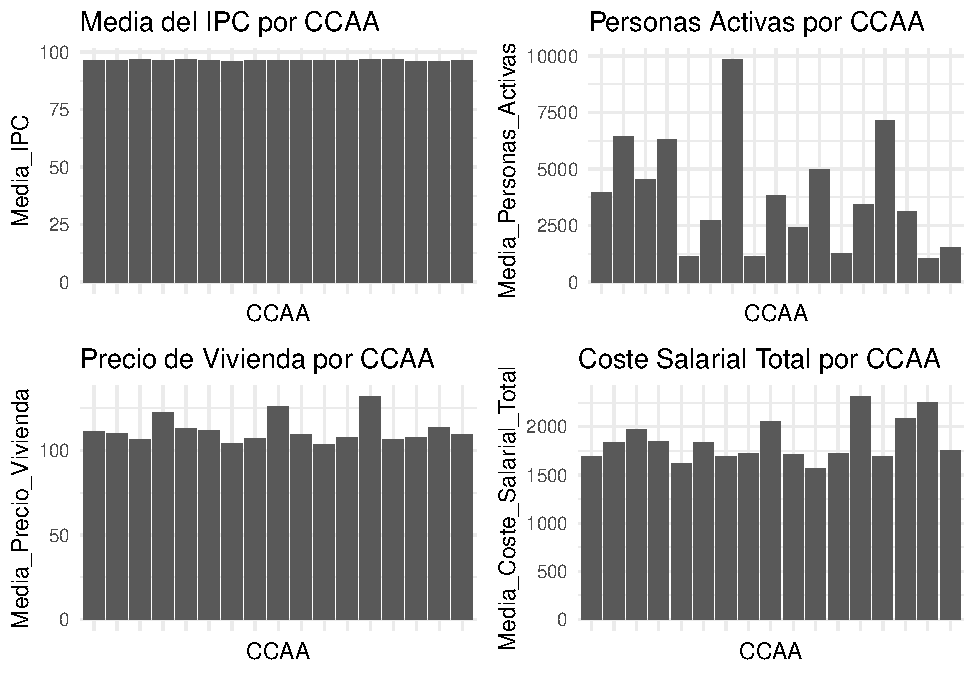
\includegraphics{trabajo_files/figure-latex/unnamed-chunk-5-1.pdf}

\begin{enumerate}
\def\labelenumi{\arabic{enumi}.}
\item
  \textbf{Evolución Media del IPC}: Las barras parecen tener alturas
  similares, lo que indicaría que el IPC medio no varía
  significativamente entre las CCAA. Sin embargo, la uniformidad del IPC
  no implica necesariamente una uniformidad en los precios de la
  vivienda, ya que pueden estar afectados por factores locales
  específicos.
\item
  \textbf{Evolución de Personas Activas}: Hay una variabilidad
  considerable en el número medio de personas activas entre las CCAA.
  Esto podría reflejar diferencias en la demografía, el mercado laboral
  y la economía de las regiones. Las regiones con más personas activas
  podrían tener una mayor demanda de vivienda, lo que a su vez podría
  influir en los precios.
\item
  \textbf{Evolución del Precio de Vivienda}: Las diferencias en las
  medias del precio de vivienda entre las CCAA son notables y pueden
  reflejar la variación en la demanda de vivienda, el ingreso disponible
  y las preferencias de los consumidores. La evolución del precio de la
  vivienda es el resultado de múltiples factores, incluyendo la economía
  local, la oferta y demanda de viviendas, y las políticas de vivienda.
\item
  \textbf{Evolución del Coste Salarial Total}: Al igual que con las
  personas activas, hay una variación significativa entre las CCAA en el
  coste salarial total medio. Esto podría indicar diferencias en las
  estructuras del mercado laboral y los niveles de ingreso, lo que a su
  vez podría afectar a la capacidad de los individuos para comprar
  viviendas.
\end{enumerate}

Vamos a ver en más profundidad nuestra variable explicada, el precio de
la vivienda.

\begin{Shaded}
\begin{Highlighting}[]
\CommentTok{\# Libraries}
\FunctionTok{library}\NormalTok{(tidyverse)}
\end{Highlighting}
\end{Shaded}

\begin{verbatim}
## Warning: package 'tibble' was built under R version 4.2.3
\end{verbatim}

\begin{verbatim}
## -- Attaching core tidyverse packages ------------------------ tidyverse 2.0.0 --
## v forcats   1.0.0     v readr     2.1.4
## v lubridate 1.9.2     v stringr   1.5.0
## v purrr     1.0.1     v tibble    3.2.1
## -- Conflicts ------------------------------------------ tidyverse_conflicts() --
## x dplyr::between()     masks plm::between()
## x gridExtra::combine() masks dplyr::combine()
## x dplyr::filter()      masks stats::filter()
## x dplyr::lag()         masks plm::lag(), stats::lag()
## x dplyr::lead()        masks plm::lead()
## i Use the ]8;;http://conflicted.r-lib.org/conflicted package]8;; to force all conflicts to become errors
\end{verbatim}

\begin{Shaded}
\begin{Highlighting}[]
\FunctionTok{library}\NormalTok{(hrbrthemes)}
\end{Highlighting}
\end{Shaded}

\begin{verbatim}
## Warning: package 'hrbrthemes' was built under R version 4.2.3
\end{verbatim}

\begin{verbatim}
## NOTE: Either Arial Narrow or Roboto Condensed fonts are required to use these themes.
##       Please use hrbrthemes::import_roboto_condensed() to install Roboto Condensed and
##       if Arial Narrow is not on your system, please see https://bit.ly/arialnarrow
\end{verbatim}

\begin{Shaded}
\begin{Highlighting}[]
\FunctionTok{library}\NormalTok{(kableExtra)}
\end{Highlighting}
\end{Shaded}

\begin{verbatim}
## Warning: package 'kableExtra' was built under R version 4.2.3
\end{verbatim}

\begin{verbatim}
## Warning in !is.null(rmarkdown::metadata$output) && rmarkdown::metadata$output
## %in% : 'length(x) = 2 > 1' in coercion to 'logical(1)'
\end{verbatim}

\begin{verbatim}
## 
## Attaching package: 'kableExtra'
## 
## The following object is masked from 'package:dplyr':
## 
##     group_rows
\end{verbatim}

\begin{Shaded}
\begin{Highlighting}[]
\FunctionTok{options}\NormalTok{(}\AttributeTok{knitr.table.format =} \StringTok{"html"}\NormalTok{)}
\FunctionTok{library}\NormalTok{(babynames)}
\end{Highlighting}
\end{Shaded}

\begin{verbatim}
## Warning: package 'babynames' was built under R version 4.2.3
\end{verbatim}

\begin{Shaded}
\begin{Highlighting}[]
\FunctionTok{library}\NormalTok{(viridis)}
\end{Highlighting}
\end{Shaded}

\begin{verbatim}
## Warning: package 'viridis' was built under R version 4.2.3
\end{verbatim}

\begin{verbatim}
## Loading required package: viridisLite
\end{verbatim}

\begin{verbatim}
## Warning: package 'viridisLite' was built under R version 4.2.3
\end{verbatim}

\begin{Shaded}
\begin{Highlighting}[]
\FunctionTok{library}\NormalTok{(DT)}
\end{Highlighting}
\end{Shaded}

\begin{verbatim}
## Warning: package 'DT' was built under R version 4.2.3
\end{verbatim}

\begin{Shaded}
\begin{Highlighting}[]
\FunctionTok{library}\NormalTok{(plotly)}
\end{Highlighting}
\end{Shaded}

\begin{verbatim}
## Warning: package 'plotly' was built under R version 4.2.3
\end{verbatim}

\begin{verbatim}
## 
## Attaching package: 'plotly'
## 
## The following object is masked from 'package:ggplot2':
## 
##     last_plot
## 
## The following object is masked from 'package:stats':
## 
##     filter
## 
## The following object is masked from 'package:graphics':
## 
##     layout
\end{verbatim}

\begin{Shaded}
\begin{Highlighting}[]
\CommentTok{\# Reordenar las CCAA basándose en la media del precio de la vivienda}
\NormalTok{tmp }\OtherTok{\textless{}{-}}\NormalTok{ data }\SpecialCharTok{\%\textgreater{}\%}
  \FunctionTok{mutate}\NormalTok{(}\AttributeTok{Periodo =} \FunctionTok{as\_datetime}\NormalTok{(}\FunctionTok{sapply}\NormalTok{(Periodo, convertir\_a\_fecha))) }\SpecialCharTok{\%\textgreater{}\%}
  \FunctionTok{mutate}\NormalTok{(}\AttributeTok{CCAA =} \FunctionTok{fct\_reorder}\NormalTok{(CCAA, Precio\_vivienda, }\AttributeTok{.fun =}\NormalTok{ mean, }\AttributeTok{.desc=}\ConstantTok{TRUE}\NormalTok{))}\SpecialCharTok{\%\textgreater{}\%}
    \FunctionTok{mutate}\NormalTok{(}\AttributeTok{name2=}\NormalTok{CCAA)}

\NormalTok{p }\OtherTok{=}\NormalTok{ tmp }\SpecialCharTok{\%\textgreater{}\%}
  \FunctionTok{ggplot}\NormalTok{( }\FunctionTok{aes}\NormalTok{(}\AttributeTok{x=}\NormalTok{Periodo, }\AttributeTok{y=}\NormalTok{Precio\_vivienda)) }\SpecialCharTok{+}
    \FunctionTok{geom\_line}\NormalTok{( }\AttributeTok{data=}\NormalTok{tmp }\SpecialCharTok{\%\textgreater{}\%}\NormalTok{ dplyr}\SpecialCharTok{::}\FunctionTok{select}\NormalTok{(}\SpecialCharTok{{-}}\NormalTok{CCAA), }\FunctionTok{aes}\NormalTok{(}\AttributeTok{group=}\NormalTok{name2), }\AttributeTok{color=}\StringTok{"grey"}\NormalTok{, }\AttributeTok{size=}\FloatTok{0.5}\NormalTok{, }\AttributeTok{alpha=}\FloatTok{0.5}\NormalTok{) }\SpecialCharTok{+}
    \FunctionTok{geom\_line}\NormalTok{( }\FunctionTok{aes}\NormalTok{(}\AttributeTok{color=}\NormalTok{CCAA), }\AttributeTok{color=}\StringTok{"\#69b3a2"}\NormalTok{, }\AttributeTok{size=}\FloatTok{1.2}\NormalTok{ )}\SpecialCharTok{+}
    \FunctionTok{scale\_color\_viridis}\NormalTok{(}\AttributeTok{discrete =} \ConstantTok{TRUE}\NormalTok{) }\SpecialCharTok{+}
    \FunctionTok{theme}\NormalTok{(}
      \AttributeTok{legend.position=}\StringTok{"none"}\NormalTok{,}
      \AttributeTok{plot.title =} \FunctionTok{element\_text}\NormalTok{(}\AttributeTok{size=}\DecValTok{14}\NormalTok{),}
      \AttributeTok{panel.grid =} \FunctionTok{element\_blank}\NormalTok{()}
\NormalTok{    ) }\SpecialCharTok{+}
    \FunctionTok{ggtitle}\NormalTok{(}\StringTok{"Evolución del precio de la vivienda por CCAA"}\NormalTok{) }\SpecialCharTok{+}
    \FunctionTok{facet\_wrap}\NormalTok{(}\SpecialCharTok{\textasciitilde{}}\NormalTok{CCAA)}
\end{Highlighting}
\end{Shaded}

\begin{verbatim}
## Warning: Using `size` aesthetic for lines was deprecated in ggplot2 3.4.0.
## i Please use `linewidth` instead.
## This warning is displayed once every 8 hours.
## Call `lifecycle::last_lifecycle_warnings()` to see where this warning was
## generated.
\end{verbatim}

\begin{Shaded}
\begin{Highlighting}[]
\NormalTok{p}
\end{Highlighting}
\end{Shaded}

\begin{verbatim}
## Warning: Combining variables of class <pseries> and <factor> was deprecated in ggplot2
## 3.4.0.
## i Please ensure your variables are compatible before plotting (location:
##   `join_keys()`)
## This warning is displayed once every 8 hours.
## Call `lifecycle::last_lifecycle_warnings()` to see where this warning was
## generated.
\end{verbatim}

\includegraphics{trabajo_files/figure-latex/unnamed-chunk-6-1.pdf}

En este conjunto de gráficos, realizamos una exploración visual de la
dinámica del precio de la vivienda en las Comunidades Autónomas de
España entre 2017 y 2019. El gráfico facilita una comparación inmediata
entre comunidades al resaltar la trayectoria de una comunidad específica
en cada panel, mientras se muestra el contexto proporcionado por las
demás comunidades en un plano secundario.

Observamos una tendencia general al alza en los precios de la vivienda a
lo largo del periodo estudiado, lo que podría estar en línea con un
entorno de recuperación económica, condiciones favorables de
financiamiento y posiblemente una demanda creciente impulsada por
factores demográficos y de mercado.

Algunos puntos destacables incluyen:

\begin{itemize}
\item
  \textbf{Madrid y Cataluña}: Estas comunidades muestran una marcada
  tendencia alcista en los precios de la vivienda, superando a la
  mayoría de las otras regiones. Esto podría reflejar su condición de
  centros económicos y culturales, con una demanda de vivienda robusta.
\item
  \textbf{Variabilidad entre Comunidades}: Aunque la tendencia general
  es al alza, la variabilidad en la tasa de crecimiento es notable.
  Comunidades como Extremadura y Castilla-La Mancha muestran un
  crecimiento más moderado, lo que podría sugerir diferencias en las
  presiones del mercado local o en la actividad económica.
\end{itemize}

Estos gráficos muestran que si que existen diferencias entre comunidades
a pesar de que la evolución es más o menos igual para toda españa. A
continuación, vamos a tratar de resolver las preguntas formuladas
anteriormente.

\hypertarget{modelos-de-datos-de-panel}{%
\subsection{Modelos de datos de panel}\label{modelos-de-datos-de-panel}}

Como la pregunta que nos planteamos es como influye el ipc, el coste
salarial total y el número de personas activas en el precio de la
vivienda, los modelos que se trabajarán a continuación tendrá como
variable dependiente el precio de la vivienda y como variable
independiente el número de personas activas, el ipc y el coste salarial
total.

A continuación, vamos a estimar los distintos modelos e interpretar los
coeficientes.

\begin{itemize}
\tightlist
\item
  Modelo de pool de datos
\item
  Efectos fijos individuales MCVD
\item
  Efectos aleatorios
\end{itemize}

Una vez hechos los modelos, elegiremos tanto desde el punto de vista
teórico como con los contrastes de homogeneidad y de Hausman que modelo
describe mejor el precio de la vivienda.

\hypertarget{modelo-pool-de-datos}{%
\subsubsection{Modelo Pool de datos}\label{modelo-pool-de-datos}}

Un modelo de pool de datos (pooled data model) es una técnica
estadística utilizada en econometría que combina datos de corte
transversal y series temporales para analizar y estimar efectos que son
constantes a través del tiempo pero pueden variar entre unidades
transversales.

\begin{Shaded}
\begin{Highlighting}[]
\NormalTok{pool\_datos }\OtherTok{\textless{}{-}} \FunctionTok{plm}\NormalTok{(Precio\_vivienda }\SpecialCharTok{\textasciitilde{}}\NormalTok{ Personas\_activas }\SpecialCharTok{+}\NormalTok{ IPC }\SpecialCharTok{+}\NormalTok{ Coste\_salarial\_total, }\AttributeTok{data =}\NormalTok{ data, }\AttributeTok{model =} \StringTok{"pooling"}\NormalTok{)}

\FunctionTok{summary}\NormalTok{(pool\_datos)}
\end{Highlighting}
\end{Shaded}

\begin{verbatim}
## Pooling Model
## 
## Call:
## plm(formula = Precio_vivienda ~ Personas_activas + IPC + Coste_salarial_total, 
##     data = data, model = "pooling")
## 
## Balanced Panel: n = 17, T = 12, N = 204
## 
## Residuals:
##      Min.   1st Qu.    Median   3rd Qu.      Max. 
## -13.52736  -4.72225  -0.31311   3.08416  20.79708 
## 
## Coefficients:
##                         Estimate  Std. Error t-value  Pr(>|t|)    
## (Intercept)          -1.6969e+02  3.9147e+01 -4.3346 2.312e-05 ***
## Personas_activas     -7.3953e-05  2.0316e-04 -0.3640    0.7162    
## IPC                   2.5965e+00  4.1746e-01  6.2198 2.856e-09 ***
## Coste_salarial_total  1.7343e-02  2.2138e-03  7.8338 2.732e-13 ***
## ---
## Signif. codes:  0 '***' 0.001 '**' 0.01 '*' 0.05 '.' 0.1 ' ' 1
## 
## Total Sum of Squares:    16593
## Residual Sum of Squares: 9652.2
## R-Squared:      0.41828
## Adj. R-Squared: 0.40955
## F-statistic: 47.936 on 3 and 200 DF, p-value: < 2.22e-16
\end{verbatim}

\begin{itemize}
\item
  El interceptse estima en -169.69, lo que sería el precio de la
  vivienda cuando las variables predictoras son cero, aunque este
  escenario es teóricamente no plausible.
\item
  La variable `Personas\_activas' tiene un impacto negativo
  insignificante en el precio de la vivienda (p-valor = 0.7162),
  indicando que no es un predictor estadísticamente significativo.
\item
  El `IPC' muestra un efecto positivo significativo (coeficiente =
  2.5965, p-valor \textless{} 0.001), sugiriendo que un aumento en el
  IPC se asocia con un incremento en el precio de la vivienda.
\item
  El `Coste\_salarial\_total' también es un predictor positivo y
  significativo (coeficiente = 0.017343, p-valor \textless{} 0.001),
  indicando que los aumentos en el coste salarial están asociados con
  precios de vivienda más altos.
\item
  El modelo es estadísticamente significativo en su conjunto
  (F-statistic = 47.936, p-valor \textless{} 2.22e-16) y explica
  aproximadamente el 41.83\% de la variabilidad del precio de la
  vivienda (R-cuadrado ajustado = 0.40955).
\end{itemize}

En resumen, el modelo sugiere que el IPC y el Coste Salarial Total son
variables significativas y positivas en la explicación del precio de la
vivienda, mientras que la variable ``Personas\_activas'' no parece tener
un impacto significativo.

\hypertarget{efectos-fijos-individuales-mcvd}{%
\subsubsection{Efectos fijos individuales
MCVD}\label{efectos-fijos-individuales-mcvd}}

El modelo de efectos fijos individuales controla la heterogeneidad no
observada que es constante en el tiempo pero varía entre individuos.
Mientras que el modelo de pool de datos asume que esta heterogeneidad no
observada es inexistente o irrelevante. En nuestro caso los individuos
serán las comunidades autónomas.

\begin{Shaded}
\begin{Highlighting}[]
\NormalTok{efectos\_fijos }\OtherTok{\textless{}{-}} \FunctionTok{plm}\NormalTok{(Precio\_vivienda }\SpecialCharTok{\textasciitilde{}}\NormalTok{ Personas\_activas }\SpecialCharTok{+}\NormalTok{ IPC }\SpecialCharTok{+}\NormalTok{ Coste\_salarial\_total }\SpecialCharTok{+} \FunctionTok{as.factor}\NormalTok{(CCAA), }\AttributeTok{data =}\NormalTok{ data, }\AttributeTok{model=}\StringTok{"pooling"}\NormalTok{)}

\FunctionTok{summary}\NormalTok{(efectos\_fijos)}
\end{Highlighting}
\end{Shaded}

\begin{verbatim}
## Pooling Model
## 
## Call:
## plm(formula = Precio_vivienda ~ Personas_activas + IPC + Coste_salarial_total + 
##     as.factor(CCAA), data = data, model = "pooling")
## 
## Balanced Panel: n = 17, T = 12, N = 204
## 
## Residuals:
##     Min.  1st Qu.   Median  3rd Qu.     Max. 
## -7.49705 -1.64374  0.12028  1.47490  8.31944 
## 
## Coefficients:
##                                               Estimate  Std. Error  t-value
## (Intercept)                                -2.8821e+02  1.7638e+01 -16.3400
## Personas_activas                            9.5502e-03  2.4564e-03   3.8879
## IPC                                         4.0500e+00  2.1200e-01  19.1041
## Coste_salarial_total                       -1.6648e-02  2.4623e-03  -6.7613
## as.factor(CCAA)Aragón                      -2.2048e+01  6.2926e+00  -3.5038
## as.factor(CCAA)Asturias, Principado de     -7.8617e+00  1.9446e+00  -4.0429
## as.factor(CCAA)Balears, Illes              -8.5391e+00  5.9565e+00  -1.4336
## as.factor(CCAA)Canarias                     2.6208e+01  7.0670e+00   3.7084
## as.factor(CCAA)Cantabria                    1.5300e+01  3.1820e+00   4.8081
## as.factor(CCAA)Castilla - La Mancha        -6.2173e+01  1.4554e+01  -4.2718
## as.factor(CCAA)Castilla y León              2.4351e+01  6.9997e+00   3.4788
## as.factor(CCAA)Cataluña                     2.1708e+01  1.3963e+00  15.5474
## as.factor(CCAA)Comunitat Valenciana         1.3315e+01  3.8790e+00   3.4325
## as.factor(CCAA)Extremadura                 -1.8521e+01  2.7024e+00  -6.8537
## as.factor(CCAA)Galicia                      2.3685e+01  6.7073e+00   3.5312
## as.factor(CCAA)Madrid, Comunidad de         3.4966e+01  2.1765e+00  16.0652
## as.factor(CCAA)Murcia, Región de           -3.6599e+01  7.8731e+00  -4.6486
## as.factor(CCAA)Navarra, Comunidad Foral de  1.1870e+01  2.3916e+00   4.9631
## as.factor(CCAA)País Vasco                   4.0464e+01  7.2380e+00   5.5905
## as.factor(CCAA)Rioja, La                    2.1847e+01  5.9921e+00   3.6460
##                                             Pr(>|t|)    
## (Intercept)                                < 2.2e-16 ***
## Personas_activas                           0.0001410 ***
## IPC                                        < 2.2e-16 ***
## Coste_salarial_total                       1.755e-10 ***
## as.factor(CCAA)Aragón                      0.0005759 ***
## as.factor(CCAA)Asturias, Principado de     7.755e-05 ***
## as.factor(CCAA)Balears, Illes              0.1533902    
## as.factor(CCAA)Canarias                    0.0002759 ***
## as.factor(CCAA)Cantabria                   3.157e-06 ***
## as.factor(CCAA)Castilla - La Mancha        3.106e-05 ***
## as.factor(CCAA)Castilla y León             0.0006286 ***
## as.factor(CCAA)Cataluña                    < 2.2e-16 ***
## as.factor(CCAA)Comunitat Valenciana        0.0007386 ***
## as.factor(CCAA)Extremadura                 1.051e-10 ***
## as.factor(CCAA)Galicia                     0.0005227 ***
## as.factor(CCAA)Madrid, Comunidad de        < 2.2e-16 ***
## as.factor(CCAA)Murcia, Región de           6.358e-06 ***
## as.factor(CCAA)Navarra, Comunidad Foral de 1.574e-06 ***
## as.factor(CCAA)País Vasco                  8.071e-08 ***
## as.factor(CCAA)Rioja, La                   0.0003466 ***
## ---
## Signif. codes:  0 '***' 0.001 '**' 0.01 '*' 0.05 '.' 0.1 ' ' 1
## 
## Total Sum of Squares:    16593
## Residual Sum of Squares: 1227.2
## R-Squared:      0.92604
## Adj. R-Squared: 0.9184
## F-statistic: 121.247 on 19 and 184 DF, p-value: < 2.22e-16
\end{verbatim}

El intercept es -288.2. Esto representa el valor estimado del precio de
la vivienda cuando todas las demás variables son cero y cuando la CCAA
es la referencia en nuestro caso Andalucía.

El coeficiente asociado a la variable ``Personas\_activas'' es 0.00955.
Es estadísticamente significativo (p-value \textless{} 0.001), y
positivo. Cada unidad de aumento en las personas activas se asocia con
un aumento de 0.00955 en el precio de la vivienda.

El coeficiente asociado al IPC es 4.05. Es estadísticamente
significativo (p-value \textless{} 0.001), y positivo. Cada unidad de
aumento en el IPC se asocia con un aumento de 4.05 en el precio de la
vivienda.

El coeficiente asociado al ``Coste\_salarial\_total'' es -0.01665. Es
estadísticamente significativo (p-value \textless{} 0.001), y negativo.
Cada unidad de aumento en el coste salarial total se asocia con una
disminución de 0.01665 en el precio de la vivienda.

Cada CCAA tiene su propio coeficiente asociado, que representa el cambio
promedio en el precio de la vivienda en esa CCAA en comparación con la
CCAA de referencia (Andalucía).

El valor F es 121.2 con un p-value muy pequeño (\textless{} 2.2e-16).
Esto sugiere que al menos una de las variables independientes o efectos
fijos es significativa en la explicación de la variabilidad en el precio
de la vivienda. El único coeficiente que no es significativo es el de
les Illes Balears. Este resultado sugiere que, según el modelo, no hay
evidencia suficiente para afirmar que las Islas Baleares tienen un
efecto significativo y diferente en el precio de la vivienda en
comparación con Andalucía.

El modelo parece tener un buen ajuste y explica una gran proporción de
la variabilidad en el precio de la vivienda. Las variables de personas
activas, IPC y coste salarial total son significativas en la predicción
del precio de la vivienda, y también hay diferencias significativas en
los precios de vivienda entre las diferentes CCAA.

\hypertarget{efectos-aleatorios}{%
\subsubsection{Efectos aleatorios}\label{efectos-aleatorios}}

El modelo de efectos aleatorios asume que las diferencias individuales
no observadas entre las individuos son aleatorias y no correlacionadas
con las variables independientes del modelo. A diferencia de los modelos
de efectos fijos, que estiman parámetros únicos para cada CCAA, el
enfoque de efectos aleatorios incorpora la heterogeneidad no observada
en el término del error.

\begin{Shaded}
\begin{Highlighting}[]
\NormalTok{efectos\_aleatorios }\OtherTok{\textless{}{-}} \FunctionTok{plm}\NormalTok{(Precio\_vivienda }\SpecialCharTok{\textasciitilde{}}\NormalTok{ Personas\_activas }\SpecialCharTok{+}\NormalTok{ IPC }\SpecialCharTok{+}\NormalTok{ Coste\_salarial\_total , }\AttributeTok{data =}\NormalTok{ data, }\AttributeTok{model =} \StringTok{"random"}\NormalTok{)}
\FunctionTok{summary}\NormalTok{(efectos\_aleatorios)}
\end{Highlighting}
\end{Shaded}

\begin{verbatim}
## Oneway (individual) effect Random Effect Model 
##    (Swamy-Arora's transformation)
## 
## Call:
## plm(formula = Precio_vivienda ~ Personas_activas + IPC + Coste_salarial_total, 
##     data = data, model = "random")
## 
## Balanced Panel: n = 17, T = 12, N = 204
## 
## Effects:
##                  var std.dev share
## idiosyncratic  6.670   2.583 0.144
## individual    39.578   6.291 0.856
## theta: 0.8823
## 
## Residuals:
##      Min.   1st Qu.    Median   3rd Qu.      Max. 
## -6.115484 -1.807198 -0.082073  1.420223 10.092501 
## 
## Coefficients:
##                         Estimate  Std. Error  z-value  Pr(>|z|)    
## (Intercept)          -2.5445e+02  1.8309e+01 -13.8972 < 2.2e-16 ***
## Personas_activas      8.5802e-05  6.7227e-04   0.1276    0.8984    
## IPC                   4.0642e+00  2.1855e-01  18.5960 < 2.2e-16 ***
## Coste_salarial_total -1.3654e-02  2.5485e-03  -5.3578 8.424e-08 ***
## ---
## Signif. codes:  0 '***' 0.001 '**' 0.01 '*' 0.05 '.' 0.1 ' ' 1
## 
## Total Sum of Squares:    5033.4
## Residual Sum of Squares: 1597.5
## R-Squared:      0.68263
## Adj. R-Squared: 0.67787
## Chisq: 430.173 on 3 DF, p-value: < 2.22e-16
\end{verbatim}

El intercept es -254.45. Este valor es la estimación del precio de la
vivienda cuando todas las demás variables son cero, y representa la
media de los interceptos individuales.

El coeficiente asociado a la variable ``Personas\_activas'' es
8.5802e-05. No es estadísticamente significativo a un nivel de confianza
del 95\% (p-value = 0.8984).

El coeficiente asociado al IPC es 4.0642. Es estadísticamente
significativo (p-value \textless{} 0.001), y positivo. Cada unidad de
aumento en el IPC se asocia con un aumento de 4.0642 en el precio de la
vivienda.

El coeficiente asociado al ``Coste\_salarial\_total'' es -0.013654. Es
estadísticamente significativo (p-value \textless{} 0.001), y negativo.
Cada unidad de aumento en el coste salarial total se asocia con una
disminución de 0.013654 en el precio de la vivienda.

El valor de chi-cuadrado es 430.173 con un p-value muy pequeño
(\textless{} 2.22e\textsuperscript{-16}). Esto sugiere que al menos una
de las variables independientes es significativa en la explicación de la
variabilidad en el precio de la vivienda.

La proporción de error idiosincrático es del 14\%, mientras que la
individual del 86\%. La proporción del 14.4\% para el efecto
idiosincrático significa que una parte relativamente pequeña de la
variabilidad total en el precio de la vivienda se debe a factores
específicos de cada observación que no están explicados por las
variables incluidas en tu modelo. Por otro lado, la proporción del
85.6\% para el efecto individual significa que la mayoría de la
variabilidad total en el precio de la vivienda se debe a diferencias
sistemáticas entre las entidades (individuos) que no están capturadas
por las variables incluidas en el modelo.

El modelo de efectos aleatorios tiene en cuenta la variabilidad no
observada específica a cada entidad (efecto individual) y la
variabilidad no observada específica a cada observación (efecto
idiosincrático). Los resultados sugieren que una parte significativa de
la variabilidad en el precio de la vivienda se debe a efectos
individuales, y las variables IPC y Coste Salarial Total son
significativas en la predicción del precio de la vivienda. La variable
Personas Activas no parece ser significativa en este modelo.

\hypertarget{elecciuxf3n-del-modelo}{%
\subsection{Elección del modelo}\label{elecciuxf3n-del-modelo}}

Desde el punto de vista teórico, entre un modelo de pool de datos y un
modelo de efectos fijos individuales eligiremos el modelo de efectos
fijos individuales porque existen diferencias en el precio de la
vivienda en cada CCAA. No es lo mismo el precio de la vivienda en Madrid
que en Castilla-La-Mancha o Extremadura.

Y entre un modelo de efectso fijos o aleatorios, elegiremos el modelo de
efectos fijos ya que la muestra no es aleatoria.

Desde el punto de vista de los contrastes, aplicamos en primer lugar el
contraste de homogeneidad para elegir entre pool de datos o efectos
fijos.

H0: no hay diferencias entre los individuos, todas las alfas son iguales
H1: Hay diferencias entre individuos, y por tanto es preferible tenerlas
en cuenta

\begin{Shaded}
\begin{Highlighting}[]
\FunctionTok{pFtest}\NormalTok{(efectos\_fijos, pool\_datos)}
\end{Highlighting}
\end{Shaded}

\begin{verbatim}
## 
##  F test for individual effects
## 
## data:  Precio_vivienda ~ Personas_activas + IPC + Coste_salarial_total +  ...
## F = 78.947, df1 = 16, df2 = 184, p-value < 2.2e-16
## alternative hypothesis: significant effects
\end{verbatim}

Como el p-valor \textless{} 0.05, rechazamos H0 y por tanto existirán
diferencias entre los individuos y nos quedaremos con el modelo de
efectos fijos.

A continuación, comparamos el modelo de efectos fijos con el modelo de
efectos aleatorios con el test de Hausman

H0: No hay diferencias entre los estimadores por EF o EA, beta de
efectos fijos = beta de efectos aleatorios H1: Hay diferencias entre
estimadores, probablemente porque los EA estén correlacionados con las
regresoras, beta de efectos fijos distinto beta de efectos aleatorios

\begin{Shaded}
\begin{Highlighting}[]
\FunctionTok{phtest}\NormalTok{(efectos\_fijos, efectos\_aleatorios)}
\end{Highlighting}
\end{Shaded}

\begin{verbatim}
## 
##  Hausman Test
## 
## data:  Precio_vivienda ~ Personas_activas + IPC + Coste_salarial_total +  ...
## chisq = 15.011, df = 3, p-value = 0.001807
## alternative hypothesis: one model is inconsistent
\end{verbatim}

Como el p-valor \textless{} 0.05, rechazamos H0 y por tanto existirán
diferencias entre los estimadores y nos quedaremos con el modelo de
efectos fijos.

Se puede concluir, que el modelo que mejor explica el precio de la
vivienda es el modelo de efectos fijos individuales MCVD.

\hypertarget{series-temporales}{%
\section{Series temporales}\label{series-temporales}}

En esta segunda parte del estudio, nos enfocamos en el análisis del
precio de la vivienda en la Comunidad Valenciana como una serie
temporal. Abarcamos desde el 2007 hasta la actualidad (tercer trimestre
de 2023) con una granularidad trimestral. Este período es especialmente
significativo, ya que incluye tanto el impacto de la crisis financiera
global de 2008 como las fluctuaciones económicas subsiguientes,
incluyendo la reciente pandemia de COVID-19. Durante el análisis vamos a
descubrir la naturaleza de la serie y vamos a tratar de diseñar un
modelo econométrico que prediga el índice del precio de la vivienda.
Esto nos permitirá adelantarnos al mercado de bienes raices y saber el
estado del mismo. En nuestro caso queremos ser capaces de realizar muy
buenas predicciones a un cuatrimestre vista y a medio largo plazo.

Debido a que vamos a cambiar ligeramente nuestra fuente de datos
volvermos a realizar una análisis descriptivo para entender el
comportamietno del mercado. Seguidamente, aplicaremos los análisis de
series temporales aprendidos durante el curso y alguno extra para
conseguir un modelo de predicción lo más exacto posible. Es posible que
acabemos con dos modelos predictivos y que uno prediga bien a corto
plazo y otro a medio plazo.

\hypertarget{carga-de-datos-1}{%
\subsection{Carga de datos}\label{carga-de-datos-1}}

Disponemos de los datos empleados en la parte anterior extendidos, en
concreto 57 observaciones que corresponden a todos los trimestres desde
el año 2007 hasta el tercer trimestre de 2023. Cabe recalcar que no
tenemos ningún dato faltante.

\begin{Shaded}
\begin{Highlighting}[]
\CommentTok{\# abrimos el fichero donde se encuentran nuestros datos}
\NormalTok{df }\OtherTok{\textless{}{-}} \FunctionTok{read\_excel}\NormalTok{(}\StringTok{"./precio\_vivienda\_trabajo.xlsx"}\NormalTok{)}
\end{Highlighting}
\end{Shaded}

\begin{Shaded}
\begin{Highlighting}[]
\CommentTok{\# Como los trimestres están ordenados en sentido contrario al necesario para trabajar series temporales, cambiamos el orden}
\CommentTok{\# Ordenar las filas por la columna de fechas (B)}
\NormalTok{df }\OtherTok{\textless{}{-}}\NormalTok{ df[}\FunctionTok{order}\NormalTok{(}\FunctionTok{as.character}\NormalTok{(df}\SpecialCharTok{$}\NormalTok{Periodo)), ]}
\FunctionTok{head}\NormalTok{(df)}
\end{Highlighting}
\end{Shaded}

\begin{verbatim}
## # A tibble: 6 x 2
##   Periodo Precio_vivienda
##   <chr>             <dbl>
## 1 2007T1             137.
## 2 2007T2             142.
## 3 2007T3             144.
## 4 2007T4             146.
## 5 2008T1             147.
## 6 2008T2             146.
\end{verbatim}

\hypertarget{anuxe1lisis-exploratorio-1}{%
\subsection{Análisis exploratorio}\label{anuxe1lisis-exploratorio-1}}

El primer paso de nuestro análisis es comprender la forma de nuestros
datos e identificar grandes factores socio-económicos que puedan haber
afectado. Ya que es importante identificar eventos excepcionales que
puedan alterar los datos y sesgar nuestro modelo.

\begin{Shaded}
\begin{Highlighting}[]
\CommentTok{\# Convertir periodo a fecha}
\NormalTok{df}\SpecialCharTok{$}\NormalTok{Periodo }\OtherTok{\textless{}{-}} \FunctionTok{sapply}\NormalTok{(df}\SpecialCharTok{$}\NormalTok{Periodo, convertir\_a\_fecha)}
\NormalTok{df}\SpecialCharTok{$}\NormalTok{Periodo }\OtherTok{=} \FunctionTok{as.Date}\NormalTok{(df}\SpecialCharTok{$}\NormalTok{Periodo)}
\end{Highlighting}
\end{Shaded}

\begin{Shaded}
\begin{Highlighting}[]
\FunctionTok{library}\NormalTok{(ggplot2)}

\CommentTok{\# Crear el gráfico}
\FunctionTok{ggplot}\NormalTok{(df, }\FunctionTok{aes}\NormalTok{(}\AttributeTok{x =}\NormalTok{ Periodo, }\AttributeTok{y =}\NormalTok{ Precio\_vivienda)) }\SpecialCharTok{+}
  \FunctionTok{geom\_line}\NormalTok{() }\SpecialCharTok{+}  \CommentTok{\# Línea para mostrar la evolución del precio}
  \FunctionTok{geom\_vline}\NormalTok{(}\AttributeTok{xintercept =} \FunctionTok{as.Date}\NormalTok{(}\StringTok{"2008{-}01{-}01"}\NormalTok{), }\AttributeTok{linetype =} \StringTok{"dashed"}\NormalTok{, }\AttributeTok{color =} \StringTok{"red"}\NormalTok{) }\SpecialCharTok{+}  \CommentTok{\# Línea vertical en 2012}
  \FunctionTok{annotate}\NormalTok{(}\StringTok{"text"}\NormalTok{, }\AttributeTok{x =} \FunctionTok{as.Date}\NormalTok{(}\StringTok{"2008{-}01{-}01"}\NormalTok{), }\AttributeTok{y =} \FunctionTok{max}\NormalTok{(df}\SpecialCharTok{$}\NormalTok{Precio\_vivienda), }\AttributeTok{label =} \StringTok{"Estallido burbuja"}\NormalTok{, }\AttributeTok{hjust =} \SpecialCharTok{{-}}\FloatTok{0.2}\NormalTok{, }\AttributeTok{vjust =} \DecValTok{1}\NormalTok{, }\AttributeTok{color =} \StringTok{"red"}\NormalTok{) }\SpecialCharTok{+}
  \FunctionTok{labs}\NormalTok{(}\AttributeTok{title =} \StringTok{"Evolución del Precio de la Vivienda en España (2007{-}2023)"}\NormalTok{,}
       \AttributeTok{x =} \StringTok{"Periodo"}\NormalTok{,}
       \AttributeTok{y =} \StringTok{"Precio de la Vivienda"}\NormalTok{) }\SpecialCharTok{+}
  \FunctionTok{geom\_vline}\NormalTok{(}\AttributeTok{xintercept =} \FunctionTok{as.Date}\NormalTok{(}\StringTok{"2014{-}01{-}01"}\NormalTok{), }\AttributeTok{linetype =} \StringTok{"dashed"}\NormalTok{, }\AttributeTok{color =} \StringTok{"blue"}\NormalTok{) }\SpecialCharTok{+}  \CommentTok{\# Línea vertical en 2012}
  \FunctionTok{annotate}\NormalTok{(}\StringTok{"text"}\NormalTok{, }\AttributeTok{x =} \FunctionTok{as.Date}\NormalTok{(}\StringTok{"2014{-}01{-}01"}\NormalTok{), }\AttributeTok{y =} \FunctionTok{max}\NormalTok{(df}\SpecialCharTok{$}\NormalTok{Precio\_vivienda), }\AttributeTok{label =} \StringTok{"Empieza a remontar el precio"}\NormalTok{, }\AttributeTok{hjust =} \SpecialCharTok{{-}}\FloatTok{0.05}\NormalTok{, }\AttributeTok{vjust =} \DecValTok{1}\NormalTok{, }\AttributeTok{color =} \StringTok{"blue"}\NormalTok{) }\SpecialCharTok{+}
  \FunctionTok{geom\_vline}\NormalTok{(}\AttributeTok{xintercept =} \FunctionTok{as.Date}\NormalTok{(}\StringTok{"2020{-}03{-}12"}\NormalTok{), }\AttributeTok{linetype =} \StringTok{"dashed"}\NormalTok{, }\AttributeTok{color =} \StringTok{"darkgreen"}\NormalTok{) }\SpecialCharTok{+}  \CommentTok{\# Línea vertical en 2012}
  \FunctionTok{annotate}\NormalTok{(}\StringTok{"text"}\NormalTok{, }\AttributeTok{x =} \FunctionTok{as.Date}\NormalTok{(}\StringTok{"2020{-}03{-}12"}\NormalTok{), }\AttributeTok{y =} \FunctionTok{max}\NormalTok{(df}\SpecialCharTok{$}\NormalTok{Precio\_vivienda), }\AttributeTok{label =} \StringTok{"COVID{-}19"}\NormalTok{, }\AttributeTok{hjust =} \SpecialCharTok{{-}}\FloatTok{0.1}\NormalTok{, }\AttributeTok{vjust =} \DecValTok{1}\NormalTok{, }\AttributeTok{color =} \StringTok{"darkgreen"}\NormalTok{) }\SpecialCharTok{+}
  \FunctionTok{theme\_minimal}\NormalTok{() }\SpecialCharTok{+}
  \FunctionTok{scale\_x\_date}\NormalTok{(}\AttributeTok{date\_breaks =} \StringTok{"1 year"}\NormalTok{, }\AttributeTok{date\_labels =} \StringTok{"\%Y"}\NormalTok{) }\CommentTok{\# Formato del eje X}
\end{Highlighting}
\end{Shaded}

\includegraphics{trabajo_files/figure-latex/unnamed-chunk-15-1.pdf}

La línea continua representa la serie temporal del precio, evidenciando
tres momentos críticos en el mercado inmobiliario español, marcados por
líneas verticales punteadas y anotaciones explicativas.

Primero, la línea roja punteada señala el año 2008, coincidiendo con el
estallido de la burbuja inmobiliaria. Aquí, se observa un pico seguido
de un descenso abrupto, reflejando la caída de precios post-crisis
financiera. Este fenómeno marcó el comienzo de un periodo recesivo en el
que los precios tocaron su punto más bajo el último trimestre de 2013.

Posteriormente, la línea azul punteada 2014 sugieren un punto de
inflexión donde se empieza a percibir una recuperación gradual de los
precios. Esta tendencia ascendente indica un fortalecimiento del mercado
que podría estar vinculado a mejoras en la economía española y un
incremento en la demanda de vivienda.

Finalmente, la línea punteada verde oscura resalta el impacto de la
pandemia de COVID-19 en marzo de 2020. Contrario a lo esperado, después
de un breve periodo de estancamiento, el gráfico muestra un aumento
sorprendente en los precios, lo que podría deberse a una combinación de
factores como políticas de estímulo, cambios en las preferencias de
vivienda post-confinamiento, y una bajada en las tasas de interés.

Este análisis gráfico sirve como una herramienta esencial para
comprender la dinámica del mercado inmobiliario español. A partir de lo
que vemos visto podríamos dividir la serie temporal en tres trozos
separados por el estallido de la burbuja y cuando empieza a remontar el
precio. Omitiremos el efecto de la pandemia porque no parece influir de
manera notable en la tendencia del precio.

\hypertarget{modelado-de-series-temporales}{%
\subsection{Modelado de series
temporales}\label{modelado-de-series-temporales}}

Visto el comportamiento de los datos vamos a abordar el análisis desde
dos perspectivas. En primera instancia trateremos de crear un modelo que
sea capaz de predecir el precio de la vivienda entrenandolo con todos
los datos que tenemos a nuestra disposición. Esto podría ayudar a que
nuesto modelo sepa adaptarse a cambios de tendencia. Para ello, vamos a
emplear un modelo ARIMA y calcularemos los mejores parámetros con la
función auto.arima de forecast.

Por otra parte, trataremos de conseguir un modelo de predicción
entrenandolo solo con los datos a partir de 2014, este modelo eliminará
el sesgo provocado por la burbuja y puede que sea mejor para
predicciones a medio plazo. Para este modelo utilizaremos:

\begin{itemize}
\item
  Regresión lineal
\item
  Regresión cuadrática
\item
  Regresión exponencial cuadrática
\item
  Modelos ARIMA
\end{itemize}

\hypertarget{modelo-con-todos-los-datos}{%
\subsubsection{Modelo con todos los
datos}\label{modelo-con-todos-los-datos}}

Dada la forma de los datos podríamos tratar de ajustar el modelo con una
función seno o coseno, sin embargo, además de no conocer su
implementación, la velocidad de bajada es mayor a la velocidad de subida
del precio. En carencia de una función matemática para aproximar optamos
por un modelo ARIMA.

\begin{Shaded}
\begin{Highlighting}[]
\NormalTok{df\_completo }\OtherTok{=}\NormalTok{ df}

\NormalTok{df\_completo.ts}\OtherTok{\textless{}{-}}\FunctionTok{ts}\NormalTok{(df\_completo}\SpecialCharTok{$}\NormalTok{Precio\_vivienda, }\AttributeTok{start=}\FunctionTok{c}\NormalTok{(}\DecValTok{1}\NormalTok{,}\DecValTok{1}\NormalTok{), }\AttributeTok{end=}\FunctionTok{c}\NormalTok{(}\DecValTok{17}\NormalTok{,}\DecValTok{3}\NormalTok{), }\AttributeTok{freq =} \DecValTok{4}\NormalTok{)}

\FunctionTok{autoplot}\NormalTok{(df\_completo.ts)}
\end{Highlighting}
\end{Shaded}

\includegraphics{trabajo_files/figure-latex/unnamed-chunk-16-1.pdf}

Vamos a separar nuestros datos en entrenamiento y test para luego hacer
la validación. Los datos test llegan hasta el primer trimestre de 2022.

\begin{itemize}
\item
  Datos test: {[}T1\_2007 - T1\_2022{]}
\item
  Datos validación: {[}T2\_2022 - T3\_2023{]}
\end{itemize}

\begin{Shaded}
\begin{Highlighting}[]
\NormalTok{completo\_train\_ends }\OtherTok{=} \FunctionTok{c}\NormalTok{(}\DecValTok{16}\NormalTok{,}\DecValTok{1}\NormalTok{)}
\NormalTok{completo\_valid\_starts }\OtherTok{=} \FunctionTok{c}\NormalTok{(}\DecValTok{16}\NormalTok{,}\DecValTok{2}\NormalTok{)}
\NormalTok{completo\_valid\_ends }\OtherTok{=} \FunctionTok{c}\NormalTok{(}\DecValTok{17}\NormalTok{,}\DecValTok{3}\NormalTok{)}

\NormalTok{df\_completo.ts.train}\OtherTok{\textless{}{-}}\FunctionTok{window}\NormalTok{(df\_completo.ts,}\AttributeTok{start=}\FunctionTok{c}\NormalTok{(}\DecValTok{1}\NormalTok{,}\DecValTok{1}\NormalTok{),}\AttributeTok{end=}\NormalTok{completo\_train\_ends)}
\NormalTok{df\_completo.ts.valid}\OtherTok{\textless{}{-}}\FunctionTok{window}\NormalTok{(df\_completo.ts,}\AttributeTok{start=}\NormalTok{completo\_valid\_starts,}\AttributeTok{end=}\NormalTok{completo\_valid\_ends)}
\end{Highlighting}
\end{Shaded}

\hypertarget{predicciuxf3n-a-medio-plazo}{%
\paragraph{Predicción a medio plazo}\label{predicciuxf3n-a-medio-plazo}}

\begin{Shaded}
\begin{Highlighting}[]
\NormalTok{df\_completo.autoarima}\OtherTok{\textless{}{-}}\FunctionTok{auto.arima}\NormalTok{(df\_completo.ts.train)}

\NormalTok{df\_completo.autoarima}
\end{Highlighting}
\end{Shaded}

\begin{verbatim}
## Series: df_completo.ts.train 
## ARIMA(2,2,0)(0,0,1)[4] 
## 
## Coefficients:
##           ar1      ar2    sma1
##       -0.6533  -0.2343  0.5402
## s.e.   0.1280   0.1265  0.1205
## 
## sigma^2 = 2.484:  log likelihood = -109.86
## AIC=227.72   AICc=228.46   BIC=236.03
\end{verbatim}

El modelo que nos devuelve la función auto.arima es:

\begin{enumerate}
\def\labelenumi{\arabic{enumi}.}
\item
  \textbf{Especificación del Modelo ARIMA}: La serie se ha modelado con
  un ARIMA(2,2,0)(0,0,1){[}4{]}. Esto significa que el modelo es un
  ARIMA estacional con:

  \begin{itemize}
  \item
    \textbf{AR(2)}: Dos términos autoregresivos en la parte no
    estacional del modelo, lo que sugiere que el valor actual de la
    serie está relacionado linealmente con los dos valores anteriores.
  \item
    \textbf{I(2)}: Dos diferencias no estacionales, indicando que es
    necesario diferenciar dos veces la serie para hacerla estacionaria.
  \item
    \textbf{MA(0)}: Ningún término de medias móviles en la parte no
    estacional, lo que indica que los errores (shocks o novedades) no se
    propagan a valores futuros.
  \item
    \textbf{SMA(1)}: Un término de medias móviles en la parte estacional
    con periodicidad 4, que refleja la influencia del error (shock) de
    un valor pasado estacionalmente en los valores futuros.
  \item
    \textbf{Periodicidad {[}4{]}}: El modelo identifica una
    estacionalidad en los datos con una periodicidad de 4, lo que es
    común en datos trimestrales.
  \end{itemize}
\item
  \textbf{Coeficientes}:

  \begin{itemize}
  \item
    \textbf{ar1 (-0.6533)} y \textbf{ar2 (-0.2343)}: Son los
    coeficientes de los términos autoregresivos. Ambos son negativos, lo
    que indica una relación inversa entre los precios actuales y los
    anteriores. Los errores estándar asociados (s.e.) son relativamente
    pequeños, lo que sugiere que los coeficientes son significativamente
    diferentes de cero.
  \item
    \textbf{sma1 (0.5402)}: Es el coeficiente del término de medias
    móviles estacionales. Un valor positivo sugiere que hay un efecto
    directo del error de un valor pasado en el mismo trimestre del año
    anterior.
  \end{itemize}
\item
  \textbf{Medidas de Rendimiento}:

  \begin{itemize}
  \item
    \textbf{sigma\^{}2 (2.484)}: Varianza del error del modelo, cuánto
    varían los residuos alrededor de cero.
  \item
    \textbf{log likelihood (-109.86)}: Una medida de qué tan bien el
    modelo se ajusta a los datos; cuanto más alto, mejor.
  \item
    \textbf{AIC (227.72)} y \textbf{BIC (236.03)}: Criterios de
    información que equilibran la bondad del ajuste del modelo con su
    complejidad. El modelo con el valor más bajo es preferible. AICc es
    una versión corregida del AIC para muestras pequeñas.
  \end{itemize}
\item
  \textbf{Error del Conjunto de Entrenamiento}:

  \begin{itemize}
  \item
    \textbf{ME (Media del Error)}: Casi cero, lo que indica que no hay
    sesgo en los residuos.
  \item
    \textbf{RMSE (Raíz del Error Cuadrático Medio)} y \textbf{MAE (Error
    Absoluto Medio)}: Medidas de la diferencia entre los valores
    predichos y los observados. Mientras más bajos, mejor el ajuste del
    modelo.
  \item
    \textbf{MPE (Error Porcentual Medio)} y \textbf{MAPE (Error
    Porcentual Absoluto Medio)}: Proporcionan una perspectiva del error
    en términos porcentuales. Un MAPE de 1.02\% es bastante bajo,
    indicando buen ajuste.
  \item
    \textbf{MASE (Error Absoluto Medio Escalado)}: Comparado con un
    modelo ingenuo, un MASE \textless{} 1 sugiere que el modelo tiene un
    buen rendimiento predictivo.
  \item
    \textbf{ACF1 (Primera Autocorrelación de los Residuos)}: Cercano a
    cero, lo que indica que no hay autocorrelación en los residuos y que
    el modelo está capturando adecuadamente la estructura temporal de
    los datos.
  \end{itemize}
\end{enumerate}

En resumen, los resultados indican que el modelo
ARIMA(2,2,0)(0,0,1){[}4{]} ajustado parece ser adecuado y capaz de
capturar la dinámica de la serie temporal del precio de la vivienda. Los
errores son bajos, y no parece haber un sesgo sistemático en las
predicciones del modelo.

\begin{Shaded}
\begin{Highlighting}[]
\FunctionTok{autoplot}\NormalTok{(}\FunctionTok{cbind}\NormalTok{(df\_completo.autoarima}\SpecialCharTok{$}\NormalTok{fitted,df\_completo.ts), }\AttributeTok{xlab=}\StringTok{"Año"}\NormalTok{, }\AttributeTok{ylab=}\StringTok{"Indice precio vivienda"}\NormalTok{)}
\end{Highlighting}
\end{Shaded}

\includegraphics{trabajo_files/figure-latex/unnamed-chunk-19-1.pdf}

El gráfico presenta la comparación entre los valores reales del índice
de precios de la vivienda (en azul) y las predicciones generadas por el
modelo ARIMA(2,2,0)(0,0,1){[}4{]} (en rojo) a lo largo del tiempo. Se
observa una estrecha alineación entre ambas series, indicando un ajuste
adecuado del modelo a los datos históricos.

Las predicciones del modelo capturan las tendencias y los cambios de
dirección en el índice de precios, reflejando tanto el pico pre-crisis
como el posterior declive y recuperación. Podemos observar como los
periodos con mayor error son aquellos en los que se produce un cambio de
tendencia, como en el punto en el que empiezan a remontar los precios de
la vivienda

\begin{Shaded}
\begin{Highlighting}[]
\FunctionTok{library}\NormalTok{(}\StringTok{"TSPred"}\NormalTok{)}
\end{Highlighting}
\end{Shaded}

\begin{verbatim}
## Warning: package 'TSPred' was built under R version 4.2.3
\end{verbatim}

\begin{verbatim}
## 
## Attaching package: 'TSPred'
\end{verbatim}

\begin{verbatim}
## The following object is masked from 'package:base':
## 
##     subset
\end{verbatim}

\begin{Shaded}
\begin{Highlighting}[]
\NormalTok{df\_completo.autoarima.pred.valid }\OtherTok{\textless{}{-}} \FunctionTok{forecast}\NormalTok{(df\_completo.autoarima, }\AttributeTok{h =} \FunctionTok{length}\NormalTok{(df\_completo.ts.valid))}

\FunctionTok{plotarimapred}\NormalTok{(df\_completo.ts, df\_completo.autoarima.pred.valid, }\AttributeTok{xlim=}\FunctionTok{c}\NormalTok{(}\DecValTok{1}\NormalTok{,}\DecValTok{18}\NormalTok{), }\AttributeTok{range.percent =} \FloatTok{0.001}\NormalTok{)}
\end{Highlighting}
\end{Shaded}

\includegraphics{trabajo_files/figure-latex/unnamed-chunk-20-1.pdf}

La línea de predicción parece iniciar cerca de la continuidad de la
serie real, lo que indica un buen ajuste inicial del modelo. Sin
embargo, el área de confianza se amplía progresivamente con el tiempo,
indicando un aumento en la incertidumbre de las predicciones a medida
que nos alejamos del último punto conocido. Esto se debe a que las
predicciones de los modelos ARIMA se basan en la suposición de que las
condiciones pasadas, reflejadas en la estructura autoregresiva y de
medias móviles, se mantendrán en el futuro.

Con cada nuevo paso de predicción, los errores se acumulan y la base de
información del modelo para realizar la predicción siguiente se
debilita, ya que se basa cada vez más en predicciones en lugar de en
observaciones reales. Este fenómeno es conocido como `decadencia de la
predicción'. Además, eventos futuros no anticipados por el modelo,
cambios en la tendencia subyacente, o el impacto de choques externos que
no se han incorporado en el modelo histórico, pueden contribuir a una
disminución en la precisión de las predicciones a largo plazo.

Para analizar lo bueno que es un modelo nos fijaremos en los datos test.
A continación analizamos los parámetros de bondad del modelo. Para este
trabajo vamos a utilizar un R\textsuperscript{2} un poco distinto, en
vez de ser el porcentaje de variabilidad que explica el modelo con
respecto a su media, será con respecto a una predicción ingenua. Para
calcularlo modificaremos la suma de cuadrados total, en lugar de
calcularla con la media lo haremos con la última predicción de los datos
test. De esta forma, podremos comparar fácilmente cuanto mejor es
nuestro modelo a una predicción ingenua.

\begin{Shaded}
\begin{Highlighting}[]
\NormalTok{bondad }\OtherTok{=} \ControlFlowTok{function}\NormalTok{(real, comparacion, aprox) \{}
\NormalTok{  errores }\OtherTok{=}\NormalTok{ real }\SpecialCharTok{{-}}\NormalTok{ aprox}

  \CommentTok{\# Calcula el RMSE}
\NormalTok{  rmse }\OtherTok{\textless{}{-}} \FunctionTok{sqrt}\NormalTok{(}\FunctionTok{mean}\NormalTok{(errores}\SpecialCharTok{\^{}}\DecValTok{2}\NormalTok{))}
\NormalTok{  rmse}
  
  \CommentTok{\# Calcula MAE}
\NormalTok{  mae }\OtherTok{\textless{}{-}} \FunctionTok{mean}\NormalTok{(}\FunctionTok{abs}\NormalTok{(errores))}
  
  \CommentTok{\# Calcula MAPE}
\NormalTok{  mape }\OtherTok{\textless{}{-}} \FunctionTok{mean}\NormalTok{(}\FunctionTok{abs}\NormalTok{((errores) }\SpecialCharTok{/}\NormalTok{ real)) }\SpecialCharTok{*} \DecValTok{100}


  \CommentTok{\# Calculate the total sum of squares (SST)}
\NormalTok{  sst }\OtherTok{\textless{}{-}} \FunctionTok{sum}\NormalTok{((real }\SpecialCharTok{{-}}\NormalTok{ comparacion)}\SpecialCharTok{\^{}}\DecValTok{2}\NormalTok{)}
  
  \CommentTok{\# Calculate the residual sum of squares (SSE)}
\NormalTok{  sse }\OtherTok{\textless{}{-}} \FunctionTok{sum}\NormalTok{((real }\SpecialCharTok{{-}}\NormalTok{ aprox)}\SpecialCharTok{\^{}}\DecValTok{2}\NormalTok{)}
  
  \CommentTok{\# R{-}squared is 1 {-} (SSE/SST)}
\NormalTok{  r\_squared }\OtherTok{\textless{}{-}} \DecValTok{1} \SpecialCharTok{{-}}\NormalTok{ (sse}\SpecialCharTok{/}\NormalTok{sst)}
\NormalTok{  r\_squared}
  \FunctionTok{cat}\NormalTok{(}\StringTok{\textquotesingle{}}\SpecialCharTok{\textbackslash{}n}\StringTok{\textquotesingle{}}\NormalTok{)}
  \FunctionTok{cat}\NormalTok{(}\StringTok{\textquotesingle{}MAE: \textquotesingle{}}\NormalTok{, }\FunctionTok{round}\NormalTok{(mae, }\DecValTok{6}\NormalTok{), }\StringTok{\textquotesingle{}}\SpecialCharTok{\textbackslash{}n}\StringTok{\textquotesingle{}}\NormalTok{)}
  \FunctionTok{cat}\NormalTok{(}\StringTok{\textquotesingle{}MAPE:\textquotesingle{}}\NormalTok{, }\FunctionTok{round}\NormalTok{(mape, }\DecValTok{6}\NormalTok{), }\StringTok{\textquotesingle{}}\SpecialCharTok{\textbackslash{}n}\StringTok{\textquotesingle{}}\NormalTok{)}
  \FunctionTok{cat}\NormalTok{(}\StringTok{\textquotesingle{}RMSE:\textquotesingle{}}\NormalTok{, }\FunctionTok{round}\NormalTok{(rmse, }\DecValTok{6}\NormalTok{), }\StringTok{\textquotesingle{}}\SpecialCharTok{\textbackslash{}n}\StringTok{\textquotesingle{}}\NormalTok{)}
  \FunctionTok{cat}\NormalTok{(}\StringTok{\textquotesingle{}R\^{}2*:\textquotesingle{}}\NormalTok{, }\FunctionTok{round}\NormalTok{(r\_squared, }\DecValTok{6}\NormalTok{), }\StringTok{\textquotesingle{}}\SpecialCharTok{\textbackslash{}n}\StringTok{\textquotesingle{}}\NormalTok{)}
  \FunctionTok{cat}\NormalTok{(}\StringTok{\textquotesingle{}}\SpecialCharTok{\textbackslash{}n}\StringTok{\textquotesingle{}}\NormalTok{)}
\NormalTok{\}}

\NormalTok{ultima\_observacion\_train }\OtherTok{=}\NormalTok{ (completo\_train\_ends[}\DecValTok{1}\NormalTok{] }\SpecialCharTok{{-}}\DecValTok{1}\NormalTok{) }\SpecialCharTok{*} \DecValTok{4} \SpecialCharTok{+}\NormalTok{ completo\_train\_ends[}\DecValTok{2}\NormalTok{]}

\FunctionTok{bondad}\NormalTok{(df\_completo.ts.valid, df\_completo.ts[ultima\_observacion\_train], df\_completo.autoarima.pred.valid}\SpecialCharTok{$}\NormalTok{mean)}
\end{Highlighting}
\end{Shaded}

\begin{verbatim}
## 
## MAE:  7.538861 
## MAPE: 5.609502 
## RMSE: 8.428808 
## R^2*: -0.871797
\end{verbatim}

\begin{enumerate}
\def\labelenumi{\arabic{enumi}.}
\item
  \textbf{MAE: 7.538861} - Este valor indica que, en promedio, nuestras
  predicciones se desvían por aproximadamente 7.54 unidades del valor
  real. Este nivel de error, dependiendo de la escala de los precios de
  vivienda, puede ser considerado como moderado.
\item
  \textbf{MAPE: 5.609502\%} - El error porcentual absoluto medio muestra
  que hay un error del 5.61\% en nuestras predicciones. Este indicador
  es útil para comprender el error en términos relativos y ofrece una
  perspectiva de la precisión del modelo independientemente de la escala
  de los datos.
\item
  \textbf{RMSE: 8.428808} - La raíz del error cuadrático medio sugiere
  que las predicciones suelen estar a unas 8.43 unidades de distancia
  del valor real. Dado que el RMSE penaliza más los errores grandes,
  este valor nos indica que hay variabilidad en la precisión de las
  predicciones.
\item
  \textbf{R\^{}2*: -0.871797} - Con la nueva definición, este R\^{}2
  compara el modelo con una predicción ingenua. Este valor indica que el
  modelo no está superando una predicción simple basada en la última
  observación. Esto puede ser una señal de que el modelo necesita
  mejoras, pero no necesariamente sugiere una inadecuación tan grave
  como lo haría un R\^{}2 negativo en el cálculo tradicional.
\end{enumerate}

Por lo tanto, estos resultados sugieren la necesidad de una revisión y
posible ajuste del modelo, o la exploración de enfoques alternativos que
puedan manejar mejor la incertidumbre y los cambios en las tendencias a
largo plazo. Visto que con todos los datos el modelo ARIMA para medio
plazo no es recomendable pasamos a la predicción a corto plazo.

\hypertarget{predicciuxf3n-a-corto-plazo}{%
\paragraph{Predicción a corto plazo}\label{predicciuxf3n-a-corto-plazo}}

Vamos ha crear un algoritmo que calcule a un trimestre vista y vaya
reentrenando el modelo cada vez que le entra un dato nuevo. Esto tiene
sentido porque, a pesar de estar asumiendo un coste computacional
importante solo tenemos un dato por trimestre, por lo tanto, nos lo
podemos permitir. Pero, si que vamos a respetar el tipo de ARIMA sacado
anteriormente (2, 2, 0) (0, 0, 1) {[}4{]}.

\begin{Shaded}
\begin{Highlighting}[]
\CommentTok{\# Creamos una función que calcula el modelo y hace la prediccón del siguiente trimestre al índicado.}
\NormalTok{arima\_pred1 }\OtherTok{=} \ControlFlowTok{function}\NormalTok{(ts, trimestre) \{}
\NormalTok{  ts.train }\OtherTok{=} \FunctionTok{window}\NormalTok{(ts,}\AttributeTok{start=}\FunctionTok{c}\NormalTok{(}\DecValTok{1}\NormalTok{,}\DecValTok{1}\NormalTok{),}\AttributeTok{end=}\NormalTok{trimestre)}
\NormalTok{  arima }\OtherTok{=} \FunctionTok{Arima}\NormalTok{(ts.train, }\AttributeTok{order =} \FunctionTok{c}\NormalTok{(}\DecValTok{2}\NormalTok{, }\DecValTok{2}\NormalTok{, }\DecValTok{0}\NormalTok{), }\AttributeTok{seasonal =} \FunctionTok{list}\NormalTok{(}\AttributeTok{order =} \FunctionTok{c}\NormalTok{(}\DecValTok{0}\NormalTok{, }\DecValTok{0}\NormalTok{, }\DecValTok{1}\NormalTok{),  }\AttributeTok{period =} \DecValTok{4}\NormalTok{))}
\NormalTok{  pred }\OtherTok{=} \FunctionTok{forecast}\NormalTok{(arima, }\AttributeTok{h =} \DecValTok{1}\NormalTok{)}
  \FunctionTok{return}\NormalTok{(pred)}
\NormalTok{\}}

\CommentTok{\# Creamos una función genérica que nos devuelva las predicciones y los intervalos de confianza dado un intervalo de validazión}
\NormalTok{pred1 }\OtherTok{=} \ControlFlowTok{function}\NormalTok{(df, fun, train\_starts, valid\_ends) \{}
\NormalTok{  pred\_h1 }\OtherTok{\textless{}{-}} \FunctionTok{data.frame}\NormalTok{(}
    \StringTok{"Point Forecast"} \OtherTok{=} \FunctionTok{numeric}\NormalTok{(}\DecValTok{0}\NormalTok{),}
    \StringTok{"Lo 80"} \OtherTok{=} \FunctionTok{numeric}\NormalTok{(}\DecValTok{0}\NormalTok{),}
    \StringTok{"Hi 80"} \OtherTok{=} \FunctionTok{numeric}\NormalTok{(}\DecValTok{0}\NormalTok{),}
    \StringTok{"Lo 95"} \OtherTok{=} \FunctionTok{numeric}\NormalTok{(}\DecValTok{0}\NormalTok{),}
    \StringTok{"Hi 95"} \OtherTok{=} \FunctionTok{numeric}\NormalTok{(}\DecValTok{0}\NormalTok{)}
\NormalTok{  )}
\NormalTok{  ini\_year }\OtherTok{=}\NormalTok{ train\_starts[}\DecValTok{1}\NormalTok{]}
\NormalTok{  end\_year }\OtherTok{=}\NormalTok{ valid\_ends[}\DecValTok{1}\NormalTok{]}
  \ControlFlowTok{for}\NormalTok{ (y }\ControlFlowTok{in}\NormalTok{ ini\_year}\SpecialCharTok{:}\NormalTok{end\_year)\{}
    \ControlFlowTok{for}\NormalTok{ (t }\ControlFlowTok{in} \DecValTok{1}\SpecialCharTok{:}\DecValTok{4}\NormalTok{)\{}
      \ControlFlowTok{if}\NormalTok{ ((}\SpecialCharTok{!}\NormalTok{(y }\SpecialCharTok{==}\NormalTok{ valid\_ends[}\DecValTok{1}\NormalTok{] }\SpecialCharTok{\&\&}\NormalTok{ t }\SpecialCharTok{\textgreater{}}\NormalTok{ valid\_ends[}\DecValTok{2}\NormalTok{]}\SpecialCharTok{{-}}\DecValTok{1}\NormalTok{)) }\SpecialCharTok{\&\&}
\NormalTok{           (}\SpecialCharTok{!}\NormalTok{(y }\SpecialCharTok{==}\NormalTok{ train\_starts[}\DecValTok{1}\NormalTok{] }\SpecialCharTok{\&\&}\NormalTok{ t }\SpecialCharTok{\textless{}}\NormalTok{ train\_starts[}\DecValTok{2}\NormalTok{])))\{}
\NormalTok{        p }\OtherTok{=} \FunctionTok{fun}\NormalTok{(df, }\FunctionTok{c}\NormalTok{(y, t))}
\NormalTok{        pred\_h1[}\FunctionTok{nrow}\NormalTok{(pred\_h1)}\SpecialCharTok{+}\DecValTok{1}\NormalTok{,] }\OtherTok{=} \FunctionTok{as.data.frame}\NormalTok{(p)}
\NormalTok{        \}}
\NormalTok{     \}}
\NormalTok{  \}}
\NormalTok{  pred\_h1}
\NormalTok{\}}
\end{Highlighting}
\end{Shaded}

\begin{Shaded}
\begin{Highlighting}[]
\NormalTok{autoarima.pred\_h1 }\OtherTok{=} \FunctionTok{pred1}\NormalTok{(df\_completo.ts, arima\_pred1, completo\_train\_ends, completo\_valid\_ends)}
\NormalTok{autoarima.pred\_h1.ts }\OtherTok{=} \FunctionTok{ts}\NormalTok{(autoarima.pred\_h1}\SpecialCharTok{$}\NormalTok{Point.Forecast, }\AttributeTok{start =}\NormalTok{ completo\_valid\_starts, }\AttributeTok{end =}\NormalTok{ completo\_valid\_ends, }\AttributeTok{frequency =} \DecValTok{4}\NormalTok{)}

\FunctionTok{autoplot}\NormalTok{(}\FunctionTok{cbind}\NormalTok{(df\_completo.autoarima}\SpecialCharTok{$}\NormalTok{fitted,df\_completo.ts, autoarima.pred\_h1.ts), }\AttributeTok{xlab=}\StringTok{"Año"}\NormalTok{, }\AttributeTok{ylab=}\StringTok{"Indice precio vivienda"}\NormalTok{) }\SpecialCharTok{+}
  \FunctionTok{scale\_color\_manual}\NormalTok{(}\AttributeTok{values =} \FunctionTok{c}\NormalTok{(}\StringTok{"\#E8943A"}\NormalTok{, }\StringTok{"\#566B8A"}\NormalTok{, }\StringTok{"\#E34836"}\NormalTok{))}
\end{Highlighting}
\end{Shaded}

\includegraphics{trabajo_files/figure-latex/unnamed-chunk-23-1.pdf}

\begin{Shaded}
\begin{Highlighting}[]
\FunctionTok{bondad}\NormalTok{(df\_completo.ts.valid, }\FunctionTok{mean}\NormalTok{(df\_completo.ts.valid), autoarima.pred\_h1.ts) }
\end{Highlighting}
\end{Shaded}

\begin{verbatim}
## 
## MAE:  2.042988 
## MAPE: 1.522266 
## RMSE: 2.23927 
## R^2*: 0.333522
\end{verbatim}

Al analizar la imagen del rendimiento de nuestro modelo, la línea roja
que representa las predicciones de test muestra un ajuste razonable a
los datos reales, aunque hay margen para mejorar. Los parámetros de
desempeño del modelo son:

\begin{itemize}
\item
  \textbf{MAE: 2.042988}, que indica la diferencia media entre los
  valores predichos y los reales.
\item
  \textbf{MAPE: 1.522266\%}, que refleja el porcentaje medio de error en
  las predicciones.
\item
  \textbf{RMSE:} \textbf{2.23927}, proporcionando una medida de la
  calidad del modelo en cuanto a la variabilidad de los errores de
  predicción.
\item
  \textbf{R\^{}2: 0.333522}, lo cual sugiere que nuestro modelo explica
  aproximadamente un 33.35\% de variabilidad con respecto a un modelo
  ingenuo.
\end{itemize}

Estos indicadores de desempeño nos muestran que, aunque las predicciones
son generalmente cercanas a los valores reales, debemos trabajar en la
mejora del modelo para aumentar la precisión y la capacidad explicativa
del mismo.

\hypertarget{modelo-con-los-datos-a-partir-de-2014}{%
\subsubsection{Modelo con los datos a partir de
2014}\label{modelo-con-los-datos-a-partir-de-2014}}

Después de haber analizado modelos que incluyen el rango completo de
datos históricos, ahora vamos a enfocarnos en los datos a partir de
2014. Esta fecha marca un hito significativo, ya que corresponde al
siguiente trimetre después del punto más bajo en el precio de la
vivienda.

Al limitar nuestro análisis a este periodo de tiempo más reciente,
esperamos no solo simplificar la complejidad del modelo sino también
aumentar la precisión de nuestras predicciones al concentrarnos en un
mercado inmobiliario que ha mostrado una dinámica distinta en
comparación con el comportamiento previo a 2014. Este enfoque segmentado
nos permitirá ajustar mejor nuestros modelos a las tendencias actuales.

Continuamos con nuestro plantemiento de conseguir predicciones a medio y
a corto plazo, pudiendo suponer dos modelos distintos.

Dividimos los datos en:

\begin{itemize}
\item
  Datos test: {[}T1\_2014 - T1\_2022{]}
\item
  Datos validación: {[}T2\_2022 - T3\_2023{]}
\end{itemize}

\begin{Shaded}
\begin{Highlighting}[]
\CommentTok{\# Definimos ciertas variables genéricas de nuestro análisis}
\NormalTok{train\_ends }\OtherTok{=} \FunctionTok{c}\NormalTok{(}\DecValTok{9}\NormalTok{, }\DecValTok{1}\NormalTok{)}
\NormalTok{valid\_starts }\OtherTok{=} \FunctionTok{c}\NormalTok{(}\DecValTok{9}\NormalTok{, }\DecValTok{2}\NormalTok{)}
\NormalTok{valid\_ends }\OtherTok{=} \FunctionTok{c}\NormalTok{(}\DecValTok{10}\NormalTok{, }\DecValTok{3}\NormalTok{)}
\end{Highlighting}
\end{Shaded}

\begin{Shaded}
\begin{Highlighting}[]
\NormalTok{df\_partido }\OtherTok{=}\NormalTok{ df }\SpecialCharTok{\%\textgreater{}\%} \FunctionTok{filter}\NormalTok{(}\FunctionTok{year}\NormalTok{(Periodo) }\SpecialCharTok{\textgreater{}=} \DecValTok{2014}\NormalTok{)}

\NormalTok{df\_partido.ts}\OtherTok{\textless{}{-}}\FunctionTok{ts}\NormalTok{(df\_partido}\SpecialCharTok{$}\NormalTok{Precio\_vivienda, }\AttributeTok{start=}\FunctionTok{c}\NormalTok{(}\DecValTok{1}\NormalTok{,}\DecValTok{1}\NormalTok{), }\AttributeTok{end=}\FunctionTok{c}\NormalTok{(}\DecValTok{10}\NormalTok{,}\DecValTok{3}\NormalTok{), }\AttributeTok{freq =} \DecValTok{4}\NormalTok{)}

\FunctionTok{autoplot}\NormalTok{(df\_partido.ts)}
\end{Highlighting}
\end{Shaded}

\includegraphics{trabajo_files/figure-latex/unnamed-chunk-25-1.pdf}

Este gráfico representa los datos con los que vamos a trabajar para
obtener los modelos.

\begin{Shaded}
\begin{Highlighting}[]
\NormalTok{df\_partido.ts.train}\OtherTok{\textless{}{-}}\FunctionTok{window}\NormalTok{(df\_partido.ts,}\AttributeTok{start =} \FunctionTok{c}\NormalTok{(}\DecValTok{1}\NormalTok{,}\DecValTok{1}\NormalTok{), }\AttributeTok{end =}\NormalTok{ train\_ends)}
\NormalTok{df\_partido.ts.valid}\OtherTok{\textless{}{-}}\FunctionTok{window}\NormalTok{(df\_partido.ts,}\AttributeTok{start =}\NormalTok{ valid\_starts, }\AttributeTok{end =}\NormalTok{ valid\_ends)}
\end{Highlighting}
\end{Shaded}

\hypertarget{predicciuxf3n-a-medio-plazo-1}{%
\paragraph{Predicción a medio
plazo}\label{predicciuxf3n-a-medio-plazo-1}}

En primer lugar ajustaremos una serie de funciones matemáticas que nos
permitan modelar y entender la evolución del precio de la vivienda
durante el periodo que comienza en 2014. Consideraremos tres tipos de
modelos de regresión para capturar la naturaleza de los datos: lineal,
cuadrático y exponencial cuadrático. Seguidamente, al igual que hicimos
anteriormente entrenaremos un modelo ARIMA para ver si es capaz de
mejorar las predicciones de los modelos funcionales.

\textbf{Modelo Lineal}: Este será nuestro punto de partida,
proporcionando una línea recta que representa la tendencia general de
los precios de la vivienda con el tiempo. La simplicidad del modelo
lineal lo hace útil para obtener una vista general y puede servir como
una herramienta de comparación para modelos más complejos.

\begin{Shaded}
\begin{Highlighting}[]
\NormalTok{df\_partido.lm}\OtherTok{\textless{}{-}}\FunctionTok{tslm}\NormalTok{(df\_partido.ts.train}\SpecialCharTok{\textasciitilde{}}\NormalTok{trend)}
\end{Highlighting}
\end{Shaded}

\begin{Shaded}
\begin{Highlighting}[]
\FunctionTok{autoplot}\NormalTok{(}\FunctionTok{cbind}\NormalTok{(df\_partido.lm}\SpecialCharTok{$}\NormalTok{fitted,df\_partido.ts), }\AttributeTok{xlab=}\StringTok{"Año"}\NormalTok{, }\AttributeTok{ylab=}\StringTok{"Indice precio vivienda"}\NormalTok{) }\SpecialCharTok{+} \FunctionTok{labs}\NormalTok{(}
  \AttributeTok{title =} \StringTok{"Regresión lineal"}\NormalTok{,}
  \AttributeTok{subtitle =} \StringTok{"Predicción datos test"}\NormalTok{,}
\NormalTok{)}
\end{Highlighting}
\end{Shaded}

\includegraphics{trabajo_files/figure-latex/unnamed-chunk-28-1.pdf}

\begin{Shaded}
\begin{Highlighting}[]
\NormalTok{a }\OtherTok{=}\NormalTok{ df\_partido.lm.pred.valid }\OtherTok{\textless{}{-}} \FunctionTok{forecast}\NormalTok{(df\_partido.lm, }\AttributeTok{h =} \FunctionTok{length}\NormalTok{(df\_partido.ts.valid))}

\NormalTok{d }\OtherTok{=} \FunctionTok{plotarimapred}\NormalTok{(df\_partido.ts, df\_partido.lm.pred.valid, }\AttributeTok{xlim=}\FunctionTok{c}\NormalTok{(}\DecValTok{1}\NormalTok{,valid\_ends[}\DecValTok{1}\NormalTok{]}\SpecialCharTok{+}\DecValTok{1}\NormalTok{), }\AttributeTok{range.percent =} \FloatTok{0.001}\NormalTok{)}
\end{Highlighting}
\end{Shaded}

\includegraphics{trabajo_files/figure-latex/unnamed-chunk-28-2.pdf}

\begin{Shaded}
\begin{Highlighting}[]
\NormalTok{b }\OtherTok{=} \FunctionTok{bondad}\NormalTok{(df\_partido.ts.valid, }\FunctionTok{mean}\NormalTok{(df\_partido.ts.valid), df\_partido.lm.pred.valid}\SpecialCharTok{$}\NormalTok{mean)}
\end{Highlighting}
\end{Shaded}

\begin{verbatim}
## 
## MAE:  6.776814 
## MAPE: 5.058521 
## RMSE: 6.94718 
## R^2*: -5.414901
\end{verbatim}

Al observar el primer gráfico, notamos que el modelo lineal ajustado,
representado por la línea roja, intenta capturar la tendencia central de
la serie temporal del índice de precios de la vivienda.

El segundo gráfico proporciona una visualización clara de las
predicciones generadas por el modelo de regresión lineal, incluyendo
intervalos de confianza para las proyecciones futuras, denotados por la
banda sombreada. Este modelo extiende la línea de tendencia más allá del
último punto de datos observado, y la banda de confianza se amplía a
medida que nos alejamos de los datos conocidos, reflejando el aumento de
la incertidumbre en las predicciones a futuro.

Las estadísticas de bondad de ajuste que se presentan no son buenos.
Destacamos el R\textsuperscript{2}* negativos que indica que una
predicción ingenua sería mejor.

Aunque el modelo de regresión lineal proporciona una visión general y
simplificada de la tendencia, no es adecuado para realizar predicciones
precisas en nuestro contexto. La predicción ingenua, que se limita a
proyectar el último valor conocido, resultaría en una menor variabilidad
de los errores comparado con nuestro modelo lineal.

\textbf{Modelo Cuadrático}: Ampliando el modelo lineal, el modelo
cuadrático introducirá un término de segundo grado, permitiéndonos
capturar no solo la tendencia, sino también la aceleración o
desaceleración de los precios a lo largo del tiempo. Esto podría
reflejar cambios en el mercado que no son evidentes en un ajuste lineal.

\begin{Shaded}
\begin{Highlighting}[]
\NormalTok{df\_partido.lm2}\OtherTok{\textless{}{-}}\FunctionTok{tslm}\NormalTok{(df\_partido.ts.train}\SpecialCharTok{\textasciitilde{}} \FunctionTok{I}\NormalTok{(trend}\SpecialCharTok{\^{}}\DecValTok{2}\NormalTok{) }\SpecialCharTok{+}\NormalTok{ trend)}

\CommentTok{\# Ajuste de datos entrenamiento}
\FunctionTok{autoplot}\NormalTok{(}\FunctionTok{cbind}\NormalTok{(df\_partido.lm2}\SpecialCharTok{$}\NormalTok{fitted,df\_partido.ts), }\AttributeTok{xlab=}\StringTok{"Año"}\NormalTok{, }\AttributeTok{ylab=}\StringTok{"Indice precio vivienda"}\NormalTok{) }\SpecialCharTok{+} \FunctionTok{labs}\NormalTok{(}
  \AttributeTok{title =} \StringTok{"Regresión cuadrática"}\NormalTok{,}
  \AttributeTok{subtitle =} \StringTok{"Predicción datos test"}\NormalTok{,}
\NormalTok{)}
\end{Highlighting}
\end{Shaded}

\includegraphics{trabajo_files/figure-latex/unnamed-chunk-29-1.pdf}

\begin{Shaded}
\begin{Highlighting}[]
\CommentTok{\# Ajuste datos de test}
\NormalTok{df\_partido.lm2.pred.valid }\OtherTok{\textless{}{-}} \FunctionTok{forecast}\NormalTok{(df\_partido.lm2, }\AttributeTok{h =} \FunctionTok{length}\NormalTok{(df\_partido.ts.valid))}

\FunctionTok{plotarimapred}\NormalTok{(df\_partido.ts, df\_partido.lm2.pred.valid, }\AttributeTok{xlim=}\FunctionTok{c}\NormalTok{(}\DecValTok{1}\NormalTok{,valid\_ends[}\DecValTok{1}\NormalTok{]}\SpecialCharTok{+}\DecValTok{1}\NormalTok{), }\AttributeTok{range.percent =} \FloatTok{0.001}\NormalTok{)}
\end{Highlighting}
\end{Shaded}

\includegraphics{trabajo_files/figure-latex/unnamed-chunk-29-2.pdf}

\begin{Shaded}
\begin{Highlighting}[]
\FunctionTok{bondad}\NormalTok{(df\_partido.ts.valid, }\FunctionTok{mean}\NormalTok{(df\_partido.ts.valid), df\_partido.lm2.pred.valid}\SpecialCharTok{$}\NormalTok{mean)}
\end{Highlighting}
\end{Shaded}

\begin{verbatim}
## 
## MAE:  2.933056 
## MAPE: 2.189799 
## RMSE: 3.168091 
## R^2*: -0.334038
\end{verbatim}

Para el modelo cuadrático, los estadísticos de bondad de ajuste han
mejorado con respecto al modelo lineal, lo que sugiere una mayor
precisión en la captura de la variabilidad de los precios de la
vivienda. Sin embargo, aún se observa un R² ajustado negativo, aunque
menos extremo que en el modelo lineal, lo que indica una mejora en la
capacidad del modelo para capturar la variabilidad de los datos en
comparación con un modelo ingenuo. La búsqueda de un modelo con un R²
ajustado positivo y más cercano a 1 sería ideal, ya que indicaría una
capacidad predictiva superior a la de un modelo ingenuo y una captura
efectiva de la variabilidad de los datos.

\textbf{Modelo Exponencial Cuadrático}: el modelo exponencial cuadrático
es considerablemente más complejo y nos ayudará a entender
comportamientos no lineales en los datos. Esta función puede ser
adecuada para modelar crecimientos de tendencia multiplicativa.

\begin{Shaded}
\begin{Highlighting}[]
\NormalTok{df\_partido.exp}\OtherTok{\textless{}{-}}\FunctionTok{tslm}\NormalTok{(df\_partido.ts.train}\SpecialCharTok{\textasciitilde{}}\FunctionTok{I}\NormalTok{(trend}\SpecialCharTok{\^{}}\DecValTok{2}\NormalTok{) }\SpecialCharTok{+}\NormalTok{ trend, }\AttributeTok{lambda =} \DecValTok{0}\NormalTok{)}

\CommentTok{\# Ajuste de datos entrenamiento}
\FunctionTok{autoplot}\NormalTok{(}\FunctionTok{cbind}\NormalTok{(df\_partido.exp}\SpecialCharTok{$}\NormalTok{fitted,df\_partido.ts), }\AttributeTok{xlab=}\StringTok{"Año"}\NormalTok{, }\AttributeTok{ylab=}\StringTok{"Indice precio vivienda"}\NormalTok{) }\SpecialCharTok{+} \FunctionTok{labs}\NormalTok{(}
  \AttributeTok{title =} \StringTok{"Regresión exponencial Cuadrática"}\NormalTok{,}
  \AttributeTok{subtitle =} \StringTok{"Predicción datos test"}\NormalTok{,}
\NormalTok{)}
\end{Highlighting}
\end{Shaded}

\includegraphics{trabajo_files/figure-latex/unnamed-chunk-30-1.pdf}

\begin{Shaded}
\begin{Highlighting}[]
\CommentTok{\# Ajuste datos de test}
\NormalTok{df\_partido.exp.pred.valid }\OtherTok{\textless{}{-}} \FunctionTok{forecast}\NormalTok{(df\_partido.exp, }\AttributeTok{h =} \FunctionTok{length}\NormalTok{(df\_partido.ts.valid))}

\FunctionTok{plotarimapred}\NormalTok{(df\_partido.ts, df\_partido.exp.pred.valid, }\AttributeTok{xlim=}\FunctionTok{c}\NormalTok{(}\DecValTok{1}\NormalTok{,valid\_ends[}\DecValTok{1}\NormalTok{]}\SpecialCharTok{+}\DecValTok{1}\NormalTok{), }\AttributeTok{range.percent =} \FloatTok{0.001}\NormalTok{)}
\end{Highlighting}
\end{Shaded}

\includegraphics{trabajo_files/figure-latex/unnamed-chunk-30-2.pdf}

\begin{Shaded}
\begin{Highlighting}[]
\FunctionTok{bondad}\NormalTok{(df\_partido.ts.valid, }\FunctionTok{mean}\NormalTok{(df\_partido.ts.valid), df\_partido.exp.pred.valid}\SpecialCharTok{$}\NormalTok{mean)}
\end{Highlighting}
\end{Shaded}

\begin{verbatim}
## 
## MAE:  2.556409 
## MAPE: 1.909823 
## RMSE: 2.819245 
## R^2*: -0.056425
\end{verbatim}

Con el modelo exponencial cuadrático, los estadísticos de bondad de
ajuste muestran una mejora notable en comparación con los modelos lineal
y cuadrático previamente analizados. Aunque el R² ajustado sigue siendo
negativo, está considerablemente más cerca de cero, lo que indica una
reducción en la brecha de rendimiento con respecto a un modelo ingenuo.

\textbf{Modelo ARIMA:} Avanzando en la complejidad de nuestros modelos
econométricos, nos proponemos desarrollar un modelo ARIMA, que se adapta
específicamente para analizar y prever series temporales. Para
determinar la configuración óptima de los parámetros del modelo ARIMA,
emplearemos la función auto.arima. Esta herramienta realiza una búsqueda
exhaustiva a través de diferentes combinaciones de parámetros

\begin{Shaded}
\begin{Highlighting}[]
\NormalTok{df\_partido.autoarima}\OtherTok{\textless{}{-}}\FunctionTok{auto.arima}\NormalTok{(df\_partido.ts.train)}

\FunctionTok{print}\NormalTok{(}\StringTok{"ARIMA resultante:"}\NormalTok{)}
\end{Highlighting}
\end{Shaded}

\begin{verbatim}
## [1] "ARIMA resultante:"
\end{verbatim}

\begin{Shaded}
\begin{Highlighting}[]
\NormalTok{df\_partido.autoarima}
\end{Highlighting}
\end{Shaded}

\begin{verbatim}
## Series: df_partido.ts.train 
## ARIMA(0,1,0) with drift 
## 
## Coefficients:
##        drift
##       1.0160
## s.e.  0.2045
## 
## sigma^2 = 1.382:  log likelihood = -50.07
## AIC=104.15   AICc=104.56   BIC=107.08
\end{verbatim}

\begin{Shaded}
\begin{Highlighting}[]
\CommentTok{\# Ajuste de datos entrenamiento}
\FunctionTok{autoplot}\NormalTok{(}\FunctionTok{cbind}\NormalTok{(df\_partido.autoarima}\SpecialCharTok{$}\NormalTok{fitted,df\_partido.ts), }\AttributeTok{xlab=}\StringTok{"Año"}\NormalTok{, }\AttributeTok{ylab=}\StringTok{"Indice precio vivienda"}\NormalTok{) }\SpecialCharTok{+} \FunctionTok{labs}\NormalTok{(}
  \AttributeTok{title =} \StringTok{"ARIMA (0,1,0)"}\NormalTok{,}
  \AttributeTok{subtitle =} \StringTok{"Predicción datos test"}\NormalTok{,}
\NormalTok{)}
\end{Highlighting}
\end{Shaded}

\includegraphics{trabajo_files/figure-latex/unnamed-chunk-31-1.pdf}

\begin{Shaded}
\begin{Highlighting}[]
\CommentTok{\# Ajuste datos de test}
\NormalTok{df\_partido.autoarima.pred.valid }\OtherTok{\textless{}{-}} \FunctionTok{forecast}\NormalTok{(df\_partido.autoarima, }\AttributeTok{h =} \FunctionTok{length}\NormalTok{(df\_partido.ts.valid))}

\FunctionTok{plotarimapred}\NormalTok{(df\_partido.ts, df\_partido.autoarima.pred.valid, }\AttributeTok{xlim=}\FunctionTok{c}\NormalTok{(}\DecValTok{1}\NormalTok{,valid\_ends[}\DecValTok{1}\NormalTok{]}\SpecialCharTok{+}\DecValTok{1}\NormalTok{), }\AttributeTok{range.percent =} \FloatTok{0.001}\NormalTok{)}
\end{Highlighting}
\end{Shaded}

\includegraphics{trabajo_files/figure-latex/unnamed-chunk-31-2.pdf}

\begin{Shaded}
\begin{Highlighting}[]
\FunctionTok{bondad}\NormalTok{(df\_partido.ts.valid, }\FunctionTok{mean}\NormalTok{(df\_partido.ts.valid), df\_partido.autoarima.pred.valid}\SpecialCharTok{$}\NormalTok{mean)}
\end{Highlighting}
\end{Shaded}

\begin{verbatim}
## 
## MAE:  1.960391 
## MAPE: 1.451403 
## RMSE: 2.42105 
## R^2*: 0.220923
\end{verbatim}

El modelo ARIMA(0,1,0) con deriva proporciona una aproximación
simplificada pero potente para modelar la serie temporal del índice de
precios de la vivienda en la Comunidad Valenciana. La ausencia de
términos autoregresivos (AR) y de medias móviles (MA) indica que el
modelo se basa puramente en la diferenciación de los datos (I=1) para
lograr la estacionariedad y un término de deriva para captar la
tendencia. El coeficiente de deriva de 1.0160 sugiere una tendencia
constante en el tiempo, y su error estándar de 0.2045 muestra que este
coeficiente es estadísticamente significativo. Este modelo proporciona
un enfoque sólido y mucho mejor que los otros modelos para la predicción
del índice de precios de la vivienda. Cabe resaltar que el
R\textsuperscript{2}* del modelo es el único que es superior a 0, por lo
tanto, hemos conseguido superar al modelo ingenuo.

Así pues, es obvio que el mejor modelo de esta sección es el ARIMA (0,
1, 0), por lo tanto, nos quedaremos con ese como mejor representante de
los modelos a medio plazo con todos los datos.

\hypertarget{predicciones-a-corto-plazo}{%
\paragraph{Predicciones a corto
plazo}\label{predicciones-a-corto-plazo}}

Una vez tenemos los modelos vamos a comprobar como se comportan en la
predicción a corto plazo. Para ello utilizaremos el algoritmo planteado
en el modelo con todos los datos y comprobaremos las predicciones que
nos devuelven los modelos anteriores desechando el lineal, ya que, no
captura bien la naturaleza de los datos.

\textbf{Modelo cuadrático}

\begin{Shaded}
\begin{Highlighting}[]
\NormalTok{cuad\_pred1 }\OtherTok{=} \ControlFlowTok{function}\NormalTok{(ts, trimestre) \{}
\NormalTok{  df\_partido.ts.train }\OtherTok{=} \FunctionTok{window}\NormalTok{(df\_partido.ts,}\AttributeTok{start=}\FunctionTok{c}\NormalTok{(}\DecValTok{1}\NormalTok{,}\DecValTok{1}\NormalTok{),}\AttributeTok{end=}\NormalTok{trimestre)}
\NormalTok{  df\_partido.lm2 }\OtherTok{=} \FunctionTok{tslm}\NormalTok{(df\_partido.ts.train}\SpecialCharTok{\textasciitilde{}} \FunctionTok{I}\NormalTok{(trend}\SpecialCharTok{\^{}}\DecValTok{2}\NormalTok{) }\SpecialCharTok{+}\NormalTok{ trend)}
\NormalTok{  pred }\OtherTok{=} \FunctionTok{forecast}\NormalTok{(df\_partido.lm2, }\AttributeTok{h =} \DecValTok{1}\NormalTok{)}
\NormalTok{  pred}
\NormalTok{\}}

\NormalTok{cuad.pred\_h1 }\OtherTok{=} \FunctionTok{pred1}\NormalTok{(df\_completo.ts, cuad\_pred1, train\_ends, valid\_ends)}

\NormalTok{cuad.pred\_h1.ts }\OtherTok{=} \FunctionTok{ts}\NormalTok{(cuad.pred\_h1}\SpecialCharTok{$}\NormalTok{Point.Forecast, }\AttributeTok{start =}\NormalTok{ valid\_starts, }\AttributeTok{end =}\NormalTok{ valid\_ends, }\AttributeTok{frequency =} \DecValTok{4}\NormalTok{)}


\CommentTok{\# Ajuste de datos entrenamiento}
\FunctionTok{autoplot}\NormalTok{(}\FunctionTok{cbind}\NormalTok{(df\_partido.lm2}\SpecialCharTok{$}\NormalTok{fitted.values,df\_partido.ts, cuad.pred\_h1.ts), }\AttributeTok{xlab=}\StringTok{"Año"}\NormalTok{, }\AttributeTok{ylab=}\StringTok{"Indice precio vivienda"}\NormalTok{) }\SpecialCharTok{+}
  \FunctionTok{scale\_color\_manual}\NormalTok{(}\AttributeTok{values =} \FunctionTok{c}\NormalTok{(}\StringTok{"\#E8943A"}\NormalTok{, }\StringTok{"\#566B8A"}\NormalTok{, }\StringTok{"\#E34836"}\NormalTok{))  }\SpecialCharTok{+} \FunctionTok{labs}\NormalTok{(}
  \AttributeTok{title =} \StringTok{"Modelo cuadrático"}\NormalTok{,}
  \AttributeTok{subtitle =} \StringTok{"Predicción a un trimestre vista"}\NormalTok{,}
\NormalTok{)}
\end{Highlighting}
\end{Shaded}

\includegraphics{trabajo_files/figure-latex/unnamed-chunk-32-1.pdf}

\begin{Shaded}
\begin{Highlighting}[]
\FunctionTok{bondad}\NormalTok{(df\_partido.ts.valid, }\FunctionTok{mean}\NormalTok{(df\_partido.ts.valid), cuad.pred\_h1.ts)}
\end{Highlighting}
\end{Shaded}

\begin{verbatim}
## 
## MAE:  1.744905 
## MAPE: 1.309773 
## RMSE: 2.138936 
## R^2*: 0.391909
\end{verbatim}

Con el modelo cuadrático observamos en la gráfica que las predicciones
siguen de cerca la serie temporal del índice de precios de la vivienda.
La línea roja representa las predicciones generadas por el modelo y
podemos apreciar que se alinea estrechamente con la serie real, indicada
por la línea azul. Los estadísticos de bondad del modelo revelan un
desempeño notablemente bueno en la predicción a corto plazo.

\textbf{Modelo exponencial cuadrático}

\begin{Shaded}
\begin{Highlighting}[]
\NormalTok{exp\_pred1 }\OtherTok{=} \ControlFlowTok{function}\NormalTok{(ts, trimestre) \{}
\NormalTok{  df\_partido.ts.train }\OtherTok{=} \FunctionTok{window}\NormalTok{(df\_partido.ts,}\AttributeTok{start=}\FunctionTok{c}\NormalTok{(}\DecValTok{1}\NormalTok{,}\DecValTok{1}\NormalTok{),}\AttributeTok{end=}\NormalTok{trimestre)}
\NormalTok{  df\_partido.lm2 }\OtherTok{=} \FunctionTok{tslm}\NormalTok{(df\_partido.ts.train}\SpecialCharTok{\textasciitilde{}}\FunctionTok{I}\NormalTok{(trend}\SpecialCharTok{\^{}}\DecValTok{2}\NormalTok{) }\SpecialCharTok{+}\NormalTok{ trend, }\AttributeTok{lambda =} \DecValTok{0}\NormalTok{)}
\NormalTok{  pred }\OtherTok{=} \FunctionTok{forecast}\NormalTok{(df\_partido.lm2, }\AttributeTok{h =} \DecValTok{1}\NormalTok{)}
\NormalTok{  pred}
\NormalTok{\}}

\NormalTok{exp.pred\_h1 }\OtherTok{=} \FunctionTok{pred1}\NormalTok{(df\_partido.ts, exp\_pred1, train\_ends, valid\_ends)}
\NormalTok{exp.pred\_h1.ts }\OtherTok{=} \FunctionTok{ts}\NormalTok{(exp.pred\_h1}\SpecialCharTok{$}\NormalTok{Point.Forecast, }\AttributeTok{start =}\NormalTok{ valid\_starts, }\AttributeTok{end =}\NormalTok{ valid\_ends, }\AttributeTok{frequency =} \DecValTok{4}\NormalTok{)}


\CommentTok{\# Ajuste de datos entrenamiento}
\FunctionTok{autoplot}\NormalTok{(}\FunctionTok{cbind}\NormalTok{(df\_partido.lm2}\SpecialCharTok{$}\NormalTok{fitted.values,df\_partido.ts, exp.pred\_h1.ts), }\AttributeTok{xlab=}\StringTok{"Año"}\NormalTok{, }\AttributeTok{ylab=}\StringTok{"Indice precio vivienda"}\NormalTok{) }\SpecialCharTok{+}
  \FunctionTok{scale\_color\_manual}\NormalTok{(}\AttributeTok{values =} \FunctionTok{c}\NormalTok{(}\StringTok{"\#E8943A"}\NormalTok{, }\StringTok{"\#566B8A"}\NormalTok{, }\StringTok{"\#E34836"}\NormalTok{)) }\SpecialCharTok{+} \FunctionTok{labs}\NormalTok{(}
  \AttributeTok{title =} \StringTok{"Modelo exponencial cuadrático"}\NormalTok{,}
  \AttributeTok{subtitle =} \StringTok{"Predicción a un trimestre vista"}\NormalTok{,}
\NormalTok{)}
\end{Highlighting}
\end{Shaded}

\includegraphics{trabajo_files/figure-latex/unnamed-chunk-33-1.pdf}

\begin{Shaded}
\begin{Highlighting}[]
\FunctionTok{bondad}\NormalTok{(df\_partido.ts.valid, }\FunctionTok{mean}\NormalTok{(df\_partido.ts.valid), exp.pred\_h1.ts)}
\end{Highlighting}
\end{Shaded}

\begin{verbatim}
## 
## MAE:  1.589145 
## MAPE: 1.19486 
## RMSE: 1.999377 
## R^2*: 0.468673
\end{verbatim}

Para el modelo exponencial al igual que pasaba con las predicciones a
medio plazo todos los parámetros son mejores que el modelo cuadrático.

\textbf{Arima (0,1,0):}

\begin{Shaded}
\begin{Highlighting}[]
\NormalTok{arima2\_pred1 }\OtherTok{=} \ControlFlowTok{function}\NormalTok{(ts, trimestre) \{}
\NormalTok{  df\_partido.ts.train }\OtherTok{=} \FunctionTok{window}\NormalTok{(df\_partido.ts,}\AttributeTok{start=}\FunctionTok{c}\NormalTok{(}\DecValTok{1}\NormalTok{,}\DecValTok{1}\NormalTok{),}\AttributeTok{end=}\NormalTok{trimestre)}
\NormalTok{  modelo }\OtherTok{=} \FunctionTok{Arima}\NormalTok{(df\_partido.ts.train, }\AttributeTok{order =} \FunctionTok{c}\NormalTok{(}\DecValTok{0}\NormalTok{, }\DecValTok{1}\NormalTok{, }\DecValTok{0}\NormalTok{))}
\NormalTok{  pred }\OtherTok{=} \FunctionTok{forecast}\NormalTok{(modelo, }\AttributeTok{h =} \DecValTok{1}\NormalTok{)}
\NormalTok{  pred}
\NormalTok{\}}

\NormalTok{exp.pred\_h1 }\OtherTok{=} \FunctionTok{pred1}\NormalTok{(df\_partido.ts, arima2\_pred1, train\_ends, valid\_ends)}
\NormalTok{exp.pred\_h1.ts }\OtherTok{=} \FunctionTok{ts}\NormalTok{(exp.pred\_h1}\SpecialCharTok{$}\NormalTok{Point.Forecast, }\AttributeTok{start =}\NormalTok{ valid\_starts, }\AttributeTok{end =}\NormalTok{ valid\_ends, }\AttributeTok{frequency =} \DecValTok{4}\NormalTok{)}


\CommentTok{\# Ajuste de datos entrenamiento}
\FunctionTok{autoplot}\NormalTok{(}\FunctionTok{cbind}\NormalTok{(df\_partido.autoarima}\SpecialCharTok{$}\NormalTok{fitted, df\_partido.ts, exp.pred\_h1.ts), }\AttributeTok{xlab=}\StringTok{"Año"}\NormalTok{, }\AttributeTok{ylab=}\StringTok{"Indice precio vivienda"}\NormalTok{) }\SpecialCharTok{+}
  \FunctionTok{scale\_color\_manual}\NormalTok{(}\AttributeTok{values =} \FunctionTok{c}\NormalTok{(}\StringTok{"\#E8943A"}\NormalTok{, }\StringTok{"\#566B8A"}\NormalTok{, }\StringTok{"\#E34836"}\NormalTok{)) }\SpecialCharTok{+} \FunctionTok{labs}\NormalTok{(}
  \AttributeTok{title =} \StringTok{"Modelo ARIMA (0,1,0)"}\NormalTok{,}
  \AttributeTok{subtitle =} \StringTok{"Predicción a un trimestre vista"}\NormalTok{,}
\NormalTok{)}
\end{Highlighting}
\end{Shaded}

\includegraphics{trabajo_files/figure-latex/unnamed-chunk-34-1.pdf}

\begin{Shaded}
\begin{Highlighting}[]
\FunctionTok{bondad}\NormalTok{(df\_partido.ts.valid, }\FunctionTok{mean}\NormalTok{(df\_partido.ts.valid), exp.pred\_h1.ts)}
\end{Highlighting}
\end{Shaded}

\begin{verbatim}
## 
## MAE:  1.895833 
## MAPE: 1.408711 
## RMSE: 2.275515 
## R^2*: 0.311772
\end{verbatim}

A diferencia de las predicciones a medio plazo, en este caso, el modelo
ARIMA se comporta peor que el modelo exponencial. Esta diferencia,
además de verse en el valor de los parametros de bondad, se aprecia en
las gráficas. El modelo ARIMA se ve más afectado por el sobreajuste de
entrenarlo con todos los datos disponibles. En cambio, las predicciones
del otro modelo son más constantes ya que siguen una forma clara.

\hypertarget{elecciuxf3n-de-modelos}{%
\subsection{Elección de modelos}\label{elecciuxf3n-de-modelos}}

Tras probar diversos modelos y analizar los gráficos resultantes tenemos
un representante de cada apartado.

\begin{longtable}[]{@{}
  >{\raggedright\arraybackslash}p{(\columnwidth - 4\tabcolsep) * \real{0.2763}}
  >{\raggedright\arraybackslash}p{(\columnwidth - 4\tabcolsep) * \real{0.3158}}
  >{\raggedright\arraybackslash}p{(\columnwidth - 4\tabcolsep) * \real{0.4079}}@{}}
\toprule()
\begin{minipage}[b]{\linewidth}\raggedright
Tipo de predicción
\end{minipage} & \begin{minipage}[b]{\linewidth}\raggedright
Datos de entrenamiento
\end{minipage} & \begin{minipage}[b]{\linewidth}\raggedright
Modelo
\end{minipage} \\
\midrule()
\endhead
Un trimestre vista: & Todos los datos & ARIMA(2,2,0)(0,0,1){[}4{]} \\
& A partir de 2014 & Modelo exponencial cuadrático \\
Medio plazo: & Todos los datos & ARIMA(2,2,0)(0,0,1){[}4{]} \\
& A partir de 2014 & ARIMA(0,1,0) \\
\bottomrule()
\end{longtable}

Primeramente elegimos nuestro modelo de predicción a un trimestre vista.

\begin{Shaded}
\begin{Highlighting}[]
\CommentTok{\# ARIMA}
\FunctionTok{cat}\NormalTok{(}\StringTok{"Parámetros de bondad del modelo ARIMA (2,2,0)(0,0,1)[4] con todos los datos:"}\NormalTok{)}
\end{Highlighting}
\end{Shaded}

\begin{verbatim}
## Parámetros de bondad del modelo ARIMA (2,2,0)(0,0,1)[4] con todos los datos:
\end{verbatim}

\begin{Shaded}
\begin{Highlighting}[]
\FunctionTok{bondad}\NormalTok{(df\_completo.ts.valid, }\FunctionTok{mean}\NormalTok{(df\_completo.ts.valid), autoarima.pred\_h1.ts) }
\end{Highlighting}
\end{Shaded}

\begin{verbatim}
## 
## MAE:  2.042988 
## MAPE: 1.522266 
## RMSE: 2.23927 
## R^2*: 0.333522
\end{verbatim}

\begin{Shaded}
\begin{Highlighting}[]
\CommentTok{\# Exponencial}
\FunctionTok{cat}\NormalTok{(}\StringTok{"Parámetros de bondad del modelo Exponencial Cuadrático con los datos parciales:"}\NormalTok{)}
\end{Highlighting}
\end{Shaded}

\begin{verbatim}
## Parámetros de bondad del modelo Exponencial Cuadrático con los datos parciales:
\end{verbatim}

\begin{Shaded}
\begin{Highlighting}[]
\FunctionTok{bondad}\NormalTok{(df\_partido.ts.valid, }\FunctionTok{mean}\NormalTok{(df\_partido.ts.valid), exp.pred\_h1.ts)}
\end{Highlighting}
\end{Shaded}

\begin{verbatim}
## 
## MAE:  1.895833 
## MAPE: 1.408711 
## RMSE: 2.275515 
## R^2*: 0.311772
\end{verbatim}

El modelo exponencial cuadrático muestra un \textbf{MAE} y \textbf{MAPE}
más bajos, lo que indica que, en promedio, sus predicciones son más
cercanas a los valores reales y el error porcentual es menor. Sin
embargo, el \textbf{RMSE} es ligeramente mayor en comparación con el
modelo ARIMA, lo que sugiere que puede haber algunas predicciones que se
desvíen más de los valores reales.

En cuanto al \textbf{R²}, el modelo ARIMA tiene un valor ligeramente
superior, lo que significa que es capaz de explicar una mayor proporción
de la variabilidad de los datos en comparación con el modelo exponencial
cuadrático.

Al tomar una decisión entre los dos, se debe considerar el contexto
específico de la aplicación de estos modelos. Si se valora más la
proximidad de las predicciones a los valores reales (menor error medio),
el modelo exponencial cuadrático podría ser preferible. Sin embargo, si
se busca un modelo que explique una mayor proporción de la variabilidad
de los datos y, posiblemente, sea más estable ante variaciones más
amplias, el modelo ARIMA podría ser más adecuado.

Dado que la diferencia en el \textbf{R²} entre los dos modelos es
relativamente pequeña y el modelo exponencial cuadrático presenta
mejores \textbf{MAE} y \textbf{MAPE}, este último parece ser una opción
ligeramente mejor para la predicción a un trimestre vista.

Los modelos predictivos a medio plazo presentan los siguientes
parámetros de bondad:

\begin{Shaded}
\begin{Highlighting}[]
\FunctionTok{cat}\NormalTok{(}\StringTok{"Parámetros de bondad del modelo ARIMA (2,2,0)(0,0,1)[4] con todos los datos"}\NormalTok{)}
\end{Highlighting}
\end{Shaded}

\begin{verbatim}
## Parámetros de bondad del modelo ARIMA (2,2,0)(0,0,1)[4] con todos los datos
\end{verbatim}

\begin{Shaded}
\begin{Highlighting}[]
\FunctionTok{bondad}\NormalTok{(df\_completo.ts.valid, df\_completo.ts[ultima\_observacion\_train], df\_completo.autoarima.pred.valid}\SpecialCharTok{$}\NormalTok{mean)}
\end{Highlighting}
\end{Shaded}

\begin{verbatim}
## 
## MAE:  7.538861 
## MAPE: 5.609502 
## RMSE: 8.428808 
## R^2*: -0.871797
\end{verbatim}

\begin{Shaded}
\begin{Highlighting}[]
\FunctionTok{cat}\NormalTok{(}\StringTok{"Parámetros de bondad del modelo ARIMA (0,1,0) con los datos parciales"}\NormalTok{)}
\end{Highlighting}
\end{Shaded}

\begin{verbatim}
## Parámetros de bondad del modelo ARIMA (0,1,0) con los datos parciales
\end{verbatim}

\begin{Shaded}
\begin{Highlighting}[]
\FunctionTok{bondad}\NormalTok{(df\_partido.ts.valid, }\FunctionTok{mean}\NormalTok{(df\_partido.ts.valid), df\_partido.autoarima.pred.valid}\SpecialCharTok{$}\NormalTok{mean)}
\end{Highlighting}
\end{Shaded}

\begin{verbatim}
## 
## MAE:  1.960391 
## MAPE: 1.451403 
## RMSE: 2.42105 
## R^2*: 0.220923
\end{verbatim}

La elección de un modelo para predicciones a medio plazo implica
considerar la consistencia y la precisión de las predicciones a lo largo
de un período más extenso.

Al comparar estos parámetros, el modelo ARIMA (0,1,0) supera claramente
al ARIMA (2,2,0)(0,0,1){[}4{]} en todos los aspectos. Presenta un
\textbf{MAE}, \textbf{MAPE} y \textbf{RMSE} significativamente más
bajos, lo que indica que sus predicciones son, en promedio, mucho más
cercanas a los valores reales y presentan una menor variabilidad de los
errores. Además, el \textbf{R²} positivo del modelo ARIMA (0,1,0)
contrasta fuertemente con el valor negativo del ARIMA
(2,2,0)(0,0,1){[}4{]}, lo que sugiere que el primero tiene una capacidad
predictiva mucho más fuerte.

Sin embargo, cabe resaltar que el modelo entrenado con parte de los
datos no estaría preparado para un cambio de tendencia alcista a
bajista. Por lo tanto, sería imprescindible tener en cuenta noticias y
eventos macroeconómicos, políticos y sociales para valorar la fiabilidad
de nuestra predicción. Ante un escenario de previsible estancamiento y
posterior caida del mercado inmobiliaría nuestro modelo es probable que
no se adaptara correctamente. En cuyo caso es posible que el ARIMA
entrenado con todos los datos diera mejores aproximaciones.

\hypertarget{conclusiones}{%
\subsection{Conclusiones}\label{conclusiones}}

\end{document}
